\chapter{Resultados obtenidos}
En este capítulo se habla de los resultados obtenidos durante trabajo terminal 2.
Por tal motivo en este capítulo se abordan las pruebas realizadas y las
características que tienen los niveles para ser considerados como acabados.

\section{Pruebas}
En esta sección se reportan todos los tipos de pruebas a los que se sometió el
juego para probar tanto su funcionalidad como su desempeño y el impacto que
tuvo en los jugadores.

%\section{Prueba}


\subsection{Objetivo de la prueba}
\subsection{Herramientas utilizadas durante la prueba}
\subsection{Aplicación de la prueba}
\subsection{Conclusiones de la prueba}

%\begin{table}[prueba01]
%	\centering
%	\caption{My caption}
%	\label{my-label}
%	\begin{tabular}{ll}
%		\multicolumn{2}{l}{Prueba 01} \\
%		Objetivo                  &  asdasdasd \\
%		Herramientas utilizadas   &  asdasdasd \\
%		Aplicación                &  asdasdasd \\
%		Conclusiones              &  adasdasd
%	\end{tabular}
%\end{table}

%%\subsection{Objetivo de la prueba}
%%\subsection{Herramientas utilizadas durante la prueba}
%%\subsection{Aplicación de la prueba}
%%\subsection{Conclusiones de la prueba}

\subsection{Sprite packer}
El objetivo de esta prueba es la optimización de carga de imágenes al crear paquetes de sprites, en unity conocido como sprite packer. Se usará pruebas autómaticas con la herramienta profiles de Unity.

Una parte significativa de una textura de sprite a menudo será ocupado por el espacio vacío entre los elementos gráficos y este espacio va a resultar en memoria de video gastada en el tiempo de ejecución. Para un rendimiento optimo, lo mejor es empacar gráficas de varias texturas de sprite muy juntas dentro de una misma textura conocida como un atlas. Unity proporcionar una utilidad Sprite Packer para automatizar el proceso de generar atlases del las texturas de sprite individuales.

\begin{table}[]
	\centering
	\caption{My caption}
	\label{my-label}
	\begin{tabular}{ll}
		Pre-empaquetado & Pos-empaquetado \\
	
\includegraphics[width=5cm]{imagenes/spritespack/pre/01}	& 
\includegraphics[width=5cm]{imagenes/spritespack/pos/01}                 \\
	
\includegraphics[width=5cm]{imagenes/spritespack/pre/01}	& 
\includegraphics[width=5cm]{imagenes/spritespack/pos/01}    \\
	
\includegraphics[width=5cm]{imagenes/spritespack/pre/01}	& 
\includegraphics[width=5cm]{imagenes/spritespack/pos/01}       
	    
	\end{tabular}
\end{table}

Al final podemos determinar que si existe un menor porcentaje de carga en imágenes debido al empaquetado. En este caso el empaquetado fué en sprites estáticos, una mayor percepción de carga menor se puede observar al tener un empaquetado de animaciones, recordando que un movimiento en una imagen puede contener un número determinado de cuadros por segundo. Se deduce que si ha habido una optimización.

\subsection{Mecánicas del juego}
En esta parte se incluirán las pruebas de los componentes jugables que forman parte del juego. Como se desarrollan e insteractuan a lo largo del juego.
\subsubsection{Salto del jugador}
El objetivo de la prueba consiste en verificar la condición inicial del salto, en donde debe realizarse un doble salto.
Esta es una prueba funcional del juego, la herramienta a utilizar es el mismo programa de Unity, dentro del computador.
Al aplicar la prueba se detecta un salto ilimitado de veces en el jugador, debido a que el valor de verdadero o falso para permitir un salto extra no esta siendo detectado por el método de salto. Se hace un reporte final del fallo de salto extra.
\subsubsection{Plataforma en movimiento}
El objetivo de la prueba es comprobar que funcione la plataforma con movimiento tanto horizontal como vertical como se ha determinado. La herramienta a utilizar sigue siendo dentro del computador Unity.
Como prueba dentro del funcionamiento del juego el jugador se posiciona sobre la plataforma, la plataforma se desplaza de forma adecuada y en la dirección establecida, tanto el movimiento horizontal como el movimiento vertical. Pero se detecta que el desplazamiento es independiente al personaje, por lo que el jugador debe manualmente seguir la trayectoria de la plataforma, en este caso particular, la plataforma horizontal. Mientras que en el caso de la plataforma vertical se detecta una disminución de velocidad al realizar una ascención y un aumento de velocidad al descender. Se concluye que los componentes funcionan de manera independiente en cuanto a su movimiento, la solución a proponer consistiría en un código por parte de la plataforma en movimiento que cuando detecte al jugador le aplique la misma velocidad que este realice sumándosela a la que pudiera el jugador tener en ese momento y esto sería solo al contacto de la plataforma.

\subsection{Dinámicas del juego}
En esta parte las pruebas van dirigidas a las situaciones que crea el jugador con lo que se le hes permitido dentro del videojuego.
\subsubsection{Salto bajo}
El objetivo de la prueba consiste en entender la percepción del usuario ante las acciones que realiza el personaje dentro del juego. La herramienta a utilizar es en el computador en el programa Unity. El jugador se presenta en diferentes escenarios de los niveles para que pueda moverse a voluntado propia dentro de lo que establece el juego. Las situaciones a las que se presenta el jugador abarcan saltar en plataformas estáticas, plataformas móviles, camino horizontal y camino ascendente. Al final el usuario reporta que en su propia percepción el salto o elevación del personaje es menor al que le gustaría o en algunas ocasiones al que necesita. Las soluciones a proponer consisten en aumentar la variable que controla el movimiento ascendente del jugador o la variable que controla la gravedad proporcionada en el juego.  
\subsubsection{Instrucciones del juego}
El objetivo de la prueba consiste en entender la percepción del usuario ante las acciones que realiza dentro del nivel introductorio del juego. La herramienta a utilizar es en el computador en el programa Unity. Al usuario se le presenta el nivel introductorio del juego para que termine con este mismo. Al final reporta que por prueba y error ha sabido el funcionamiento de los botones que se le presenta, según a opinión del usuario le gustaría dentro del juego una demostración o explicación de los mismos botones y lo que hacen. Al final se propone como solución dentro de los mismos diálogos explicar el funcionamiento de los botones, o el realizar un video explicativo de los botones o indicarle al usuario que realice actividades determinadas para la prueba de los botones. 
\subsubsection{Desbloqueo de personas}
El objetivo de la prueba consiste en entender la percepción del usuario ante las acciones que realiza dentro del nivel introductorio del juego. La herramienta a utilizar es en el computador en el programa Unity. Al usuario se le presenta como situación seguir avanzando al siguiente nivel dentro del nivel introductorio, donde en una parte el jugador debe desbloquear al menos cinco diálogos. El jugador reporta que aunque sea el mismo diálogo que active una y otra vez, este se contabiliza sin ningun problema. La solución a proponer es colocar una variable de verdadero y falso para indicar si el diálogo ha sido activado y así no contabilizarlo nuevamente.


\subsection{Estética del juego}
En esta parte las pruebas van dirigidas a la respuesta del jugador ante lo que se le presenta directamente como interacción dentro del juego, ya sea auditiva o visualmente.
\subsubsection{Ilustraciones de items}
El objetivo de la prueba consiste en entender la percepción del usuario ante lo que se le muestra a lo largo del juego. La herramienta a utilizar es en el computador en el programa Unity. Dentro de los niveles impares el jugador reporta un poco confuso a primera vista el item que incrementa el tonalli, al no reconocer que objeto lo representaba. El objeto a querer mostrar es una flor de vainilla, al mostrar la imagen por separado al jugador y presentarlo en un tamaño más grande el usuario reporta como comfuso las ramas u hojas de la imagen a lado de la flor. Como propuesta de solución se tiene la eliminación de las ramas u hojas de la imagen, dejando solo la flor visible o hacer mucho más grande la imagen presente en el juego.
\subsubsection{Menú principal}
El objetivo de la prueba consiste en entender la percepción del usuario ante lo que se le muestra en el menú principal. La herramienta a utilizar es en el computador en el programa Unity.
\subsection{Prueba unitaria}
Las primera prueba unitaria fue sobre los actores. En esta sección se describe
como se realiza la prueba y como se solucionan los errores encontrados a partir
de ella.

\subsubsection{Objetivo}
Verificar el funcionamiento lógico de los componentes del nivel y definir los
valores a algunos atributos para el funcionamiento correcto de algunos actores.

\subsubsection{Herramientas}
Para la realización de esta prueba se utiliza el motor gráfico de 
\textit{Unity.}

\subsubsection{Aplicación}
Para esta prueba se evalúa el comportamiento de los actores antes de su
integración a los niveles y cómo estos interactúan con el jugador. Unity permite
ver los valores que adquieren los atributos durante su ejecución, ver figura
\ref{fig:Debug01}. Así que para esta prueba basta con ejecutar la escena
base y observar cómo responden los actores.
\\
\par
Primeramente se revisa que los enemigos y las plataformas siguen sus patrones de
movimiento definidos. Después se verifica que los enemigos, obstáculos e ítems
afecten la cantidad de vida del jugador y en algunos casos su cantidad de
\textit{tonalli}. En el caso de los jefes se verifica que sus ataques no se vean
interrumpidos por nuevos ataques de la máquina de estados. En el caso particular
de obstáculos como \textit{WindCreator} se definen los intervalos de tiempo
para su correcto funcionamiento.

        \begin{figure}[h]
                \centering
                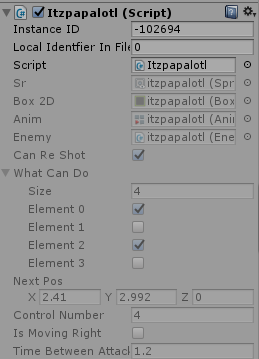
\includegraphics[width=0.2\textwidth]{04ResultadosObetnidos/imagenes/enemyPruebas01.png}
                \caption{Unity permite ver los valores de los tributos de las clases en ejecución.}
                \label{fig:Debug01}
        \end{figure}
        
\subsubsection{Resultados}
En esta prueba se observan diferentes problemas en el comportamiento de los actores
que se solucionan, a continuación se mencionan los errores encontrados y como se
solucionaron:
        \begin{itemize}
                \item El marcador se actualiza al doble cuando el jugador cae
                sobre un objeto coleccionable: Este error resulta producto de
                utilizar un \textit{GameObject} auxiliar para la detección de las
                colisiones del suelo. El error se soluciona fácilmente al agregar
                un componente de tipo rigidbody 2D al \textit{GameObject} auxiliar
                para la detección de las colisiones del suelo.
                \item Los ítems restauran el doble de vida cuando el jugador cae
                sobre ellos: Este error es generado por las mismas causas que el
                de los objetos coleccionables así que al solucionar el de los
                objetos coleccionables se soluciona éste.
                \item Los ataque de los jefes generados por corrutinas se
                empalman con otros ataques o interrumpen los que ya se están
                ejecutando: Esto se soluciona al detener todas la corrutinas generadas
                por el jefe cuando se ejecuta un ataque.
        \end{itemize}

\subsubsection{Conclusiones}
El diseño de los componentes del juego es el indicado si se desea evaluar 
componentes individuales antes de un integración completa. Esta evaluación 
de componentes agiliza la detección de errores y su corrección.
\subsection{Prueba de integración}
Esta prueba se realiza una vez se integraron los actores y controladores a los
niveles.

\subsubsection{Objetivo}
Verificar el funcionamiento lógico de los componentes del nivel al ser integrados
para formar un nivel entero.

\subsubsection{Herramientas}
Para la realización de esta prueba se utiliza el motor gráfico de \textit{Unity.}

\subsubsection{Aplicación}
Para realizar esta prueba es necesario jugar los niveles y observar que el
comportamiento de los controladores y los actores se ejecute correctamente al
integrarse con otros actores. En esta prueba también se ajustan las áreas activas de las
plataformas a fin de que su funcionamiento no se detenga si se alejan mucho del
jugador al realizar su recorrido.
                
\subsubsection{Resultados}
Al finalizar esta prueba se puede verificar que los controladores funcionan de
manera correcta; sin embargo, es necesario realizar ajustes referentes a los
tiempos de transiciones entre escenas y los valores de las áreas activas de
varias plataformas y obstáculos ya que con sus valores iniciales algunas
plataformas se detenían al realizar su recorrido dado que el jugador se salía
de su área activa y se volvía inalcanzable. En cuanto al obstáculo de
\textit{WindCreator} se ajusto el tamaño del área activa garantizando que el
obstáculo se encuentre activo cuando el jugador llegue a donde se encuentra éste. 

\subsubsection{Conclusiones}
Al finalizar esta prueba se puede concluir lo siguiente:
\begin{itemize}
    \item El desarrollo orientado a componentes facilita identificar los errores en
    las clases actoras antes de ser integradas a los niveles.
    \item Existen errores que sólo pueden ser detectados al integrar más de un actor
    y en situaciones muy específicas como el caso de los marcadores.
    \item No solo los errores de funcionamiento en el código de las clases actoras
    impactan negativamente en la experiencia del jugador; en ocasiones la experiencia
    se ve afectada por los valores que se le asignan a las clases que componen los
    actores como es el caso de los jefes y de los obstáculos.
\end{itemize} 
\subsection{Prueba de sistema}
Esta prueba se realiza una vez se integraron los actores y controladores a los
niveles. Esta orientada a la integración de las escenas entre ellas.

\subsubsection{Objetivo}
Verificar el flujo de la navegación del juego.

\subsubsection{Herramientas utilizadas durante la prueba}
Para la realización de esta prueba se utiliza el motor gráfico de \textit{Unity.}

\subsubsection{Aplicación de la prueba}
Esta prueba inicia desde la escena de menú principal en donde se verifica que
el controlador del menú realiza las validaciones correspondientes antes de
crear o cargar una partida; de igual forma se verifica que aparezcan los
mensajes de confirmación a cada caso, sea el de confirmación de la nueva partida
o el que notifica que no hay datos previamente guardados.
\\
\par
La siguiente escena a probar es el menú de selección de nivel. En este se verifica
que la información mostrada por la interfaz corresponda al nivel que se desea
acceder. Después, se verifica que en efecto el juego no permite acceder a niveles
que aún no se desbloquean.
\\
\par
Para finalizar la prueba se verifica que se realicen las transiciones entre
niveles y cinemáticas. De igual forma se prueba la funcionalidad de botones de
navegación de los niveles referentes al panel de pausa, fin de partida y nivel
completado.

\subsubsection{Conclusiones de la prueba}
Al finalizar esta prueba se pudo confirmar que las transiciones entre escenas se
realiza de manera correcta; salvo en algunos casos pero fue debido a que el nombre
de la escena a la que se debería redirigir no estaba escrito correctamente o no
coincidía con el nombre de la escena a la que debía ir. Con esto se puede concluir
que se cumple el mapa de navegación que se propuso en el documento de diseño
realizado en trabajo terminal 1.


\subsection{Prueba de rendimiento}
Esta prueba se realiza una vez que hechas las modificaciones como producto de las pruebas unitarias, de integración y de sistema.
\subsubsection{Objetivo de la prueba}
Verificar el uso del GPU. 
\subsubsection{Herramientas utilizadas durante la prueba}
\textit{Profiler de Unity.}
\subsubsection{Aplicación de la prueba}
Esta prueba inicia desde el menú principal y con la herramienta profiler se 
observa el desempeño del GPU de la maquina al simular el juego. La ventaja de utilizar 
\textit{Profiler} es que indica que elementos de la escena son los que están 
consumiendo un determinado porcentaje del GPU. En las figuras 
\ref{fig:MenuSelectionprofiler}, \ref{fig:CutSeceneprofiler} y 
\ref{fig:LevelProfiler} se muestran los resultados de la 
herramienta \textit{Profiler}.
\begin{figure}
  \centering
  
   \subfigure[Vista general del uso del GPU.] {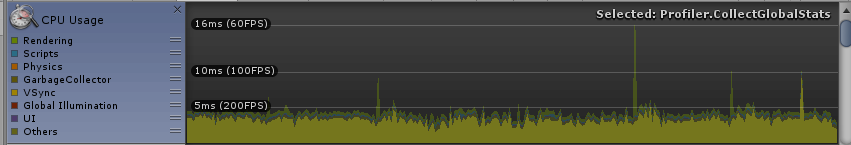
\includegraphics[width=0.6 \textwidth]
   {04ResultadosObetnidos/imagenes/ProfilerMenuselector01.png}}
   
        \subfigure[Desglose de los porcentajes del uso del GPU] {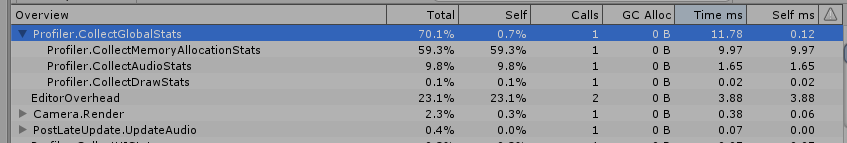
\includegraphics[width=0.6 \textwidth]{04ResultadosObetnidos/imagenes/ProfilerMenuselector02.png}}
        
        \subfigure[Desglose de los porcentajes del uso de memoria] {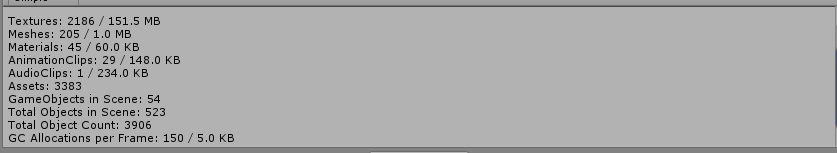
\includegraphics[width=0.6 \textwidth]{04ResultadosObetnidos/imagenes/ProfilerMenuselector04.png}}
  \caption{Resultados de la herramienta \textit{profiler} al analizar el menú de        
  seleccion.}
  \label{fig:MenuSelectionprofiler}
\end{figure} 
\begin{figure}
  \centering
  
   \subfigure[Vista general del uso del GPU.] {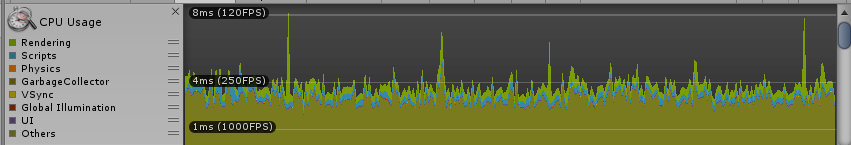
\includegraphics[width=0.6 \textwidth]
   {04ResultadosObetnidos/imagenes/cutsceneProfiler01.png}}
        
        \subfigure[Desglose de los porcentajes del uso de memoria] {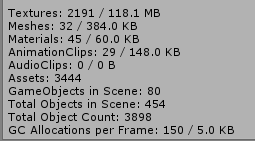
\includegraphics[width=0.3 \textwidth]{04ResultadosObetnidos/imagenes/cutsceneProfiler02.png}}
  \caption{Resultados de la herramienta \textit{profiler} al analizar una cinemática.}
  \label{fig:CutSeceneprofiler}
\end{figure} 
\begin{figure}
  \centering
  
   \subfigure[Vista general del uso del GPU.] {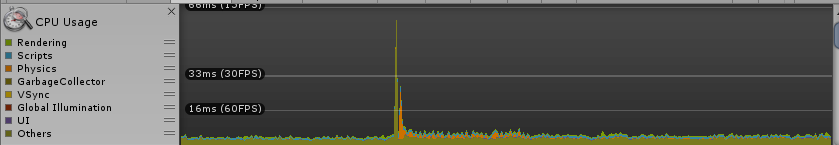
\includegraphics[width=0.6 \textwidth]
   {04ResultadosObetnidos/imagenes/Level02Profiler03.png}}
        
        \subfigure[Desglose de los porcentajes del uso del GPU] {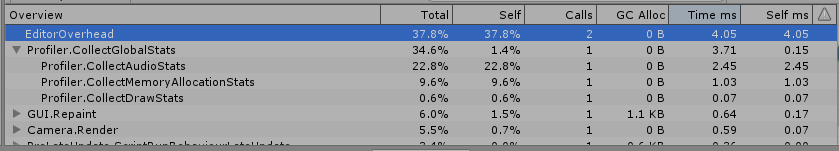
\includegraphics[width=0.6 \textwidth]{04ResultadosObetnidos/imagenes/Level02Profiler04.png}}  
        
        \subfigure[Desglose de los porcentajes del uso de memoria] {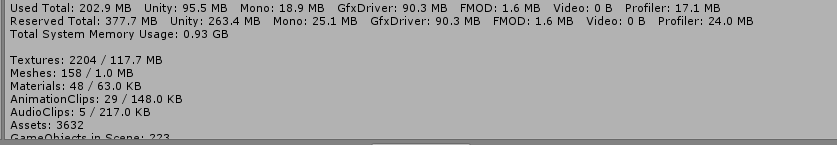
\includegraphics[width=0.6 \textwidth]{04ResultadosObetnidos/imagenes/Level02Profiler08.png}}
  \caption{Resultados de la herramienta \textit{profiler} al analizar un nivel.}
  \label{fig:LevelProfiler}
\end{figure} 
\subsubsection{Conclusiones de la prueba}
Al observar el desglose del uso del GPU en las diferentes escenas que se 
probaron, se identifica al \textit{EditorOverHead} como uno de los principales 
consumidores de recursos; investigando en la documentación de \textit{Unity}, 
se detecta que este elemento es producto de un error de rendimiento en la 
versión 2017 pero que se puede solucionar al descargar uno de los parches que 
\textit{Unity} proporciona desde su sitio web.
\\
\par
Con las pruebas de \textit{profiler} se puede concluir que el juego tiene un buen 
rendimiento en cuanto a uso de recursos puesto que no presenta caídas 
dramáticas en cuanto a desempaño.





\subsection{Prueba de rendimiento}
Esta prueba se realiza una vez que hechas las modificaciones como producto de las pruebas unitarias, de integración y de sistema.
\subsubsection{Objetivo de la prueba}
Verificar el uso del GPU y el nivel de bateria del telefono que utiliza mientras la aplicación este funcionando. 
\subsubsection{Herramientas utilizadas durante la prueba}
Opciones de desarrollador del teléfono Huawei TAG-L13 y \textit{Baterry Doctor}.
\subsubsection{Aplicación de la prueba}
Para esta prueba se debe de instalar la apk del juego en el dispositivo, activar las 
opciones de desarrollador e instalar la aplicación \textit{Baterry Doctor}.  Una vez 
hecho esto se juega el juego y se mide el desempeño desde el telefono. En las figura 
\ref{fig:GPUHuawei} se muestra el uso del GPU en distintos momentos de la 
partidad. Por otra parte en la figura \ref{fig:BateriaYolotl} se muestra el uso 
de la batería y el uso promedio de \textit{GPU} que mide \textit{Baterry Doctor}.
\\
\par
\begin{figure}
  \centering
  
   \subfigure[Uso del GPU desde el menú principal.] {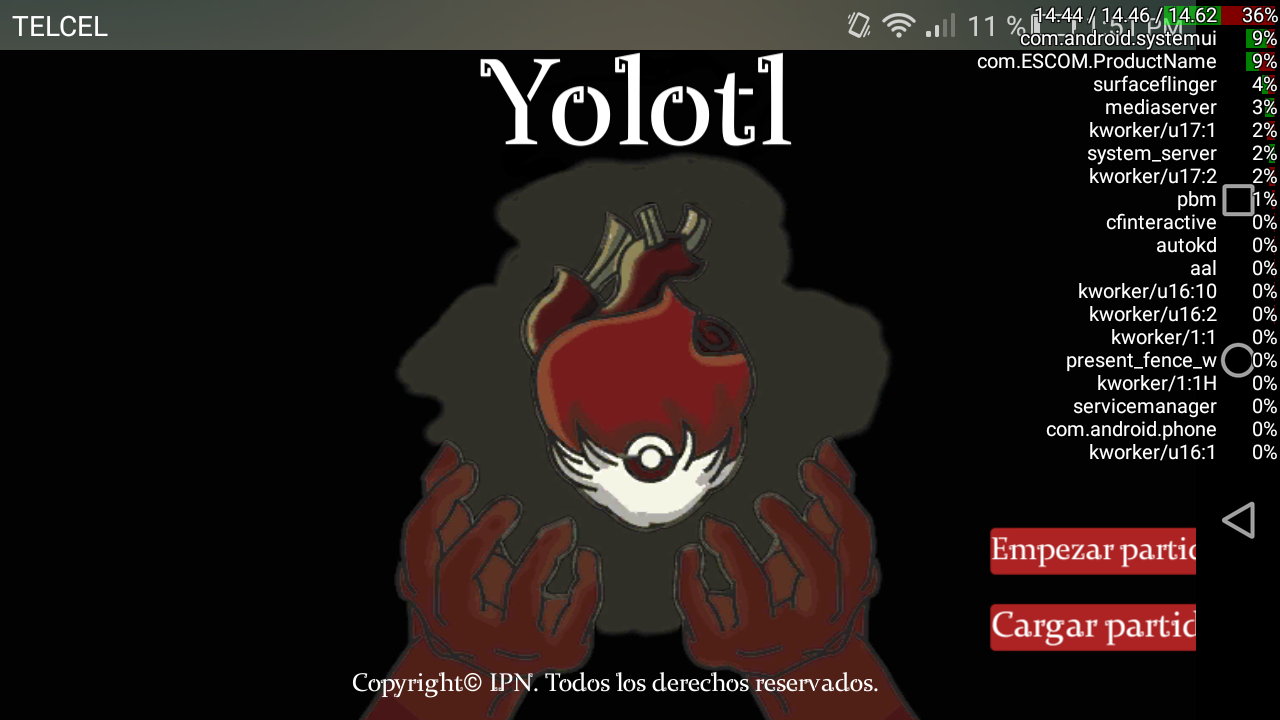
\includegraphics[width=0.4 \textwidth]{04ResultadosObetnidos/imagenes/rendimiento01.png}}
   
   \subfigure[Uso del GPU desde el menú de selección de nivel.] {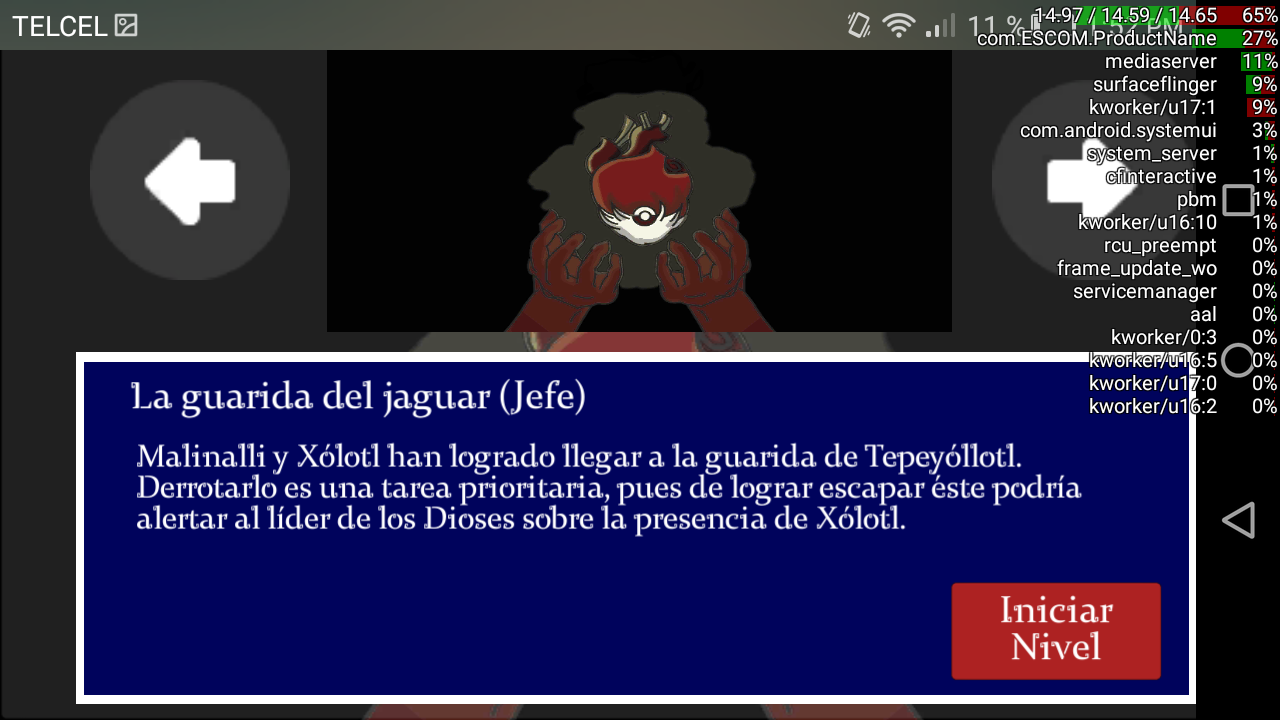
\includegraphics[width=0.4 \textwidth]{04ResultadosObetnidos/imagenes/rendimiento02.png}}
   
   \subfigure[Uso del GPU desde una cinemática.] {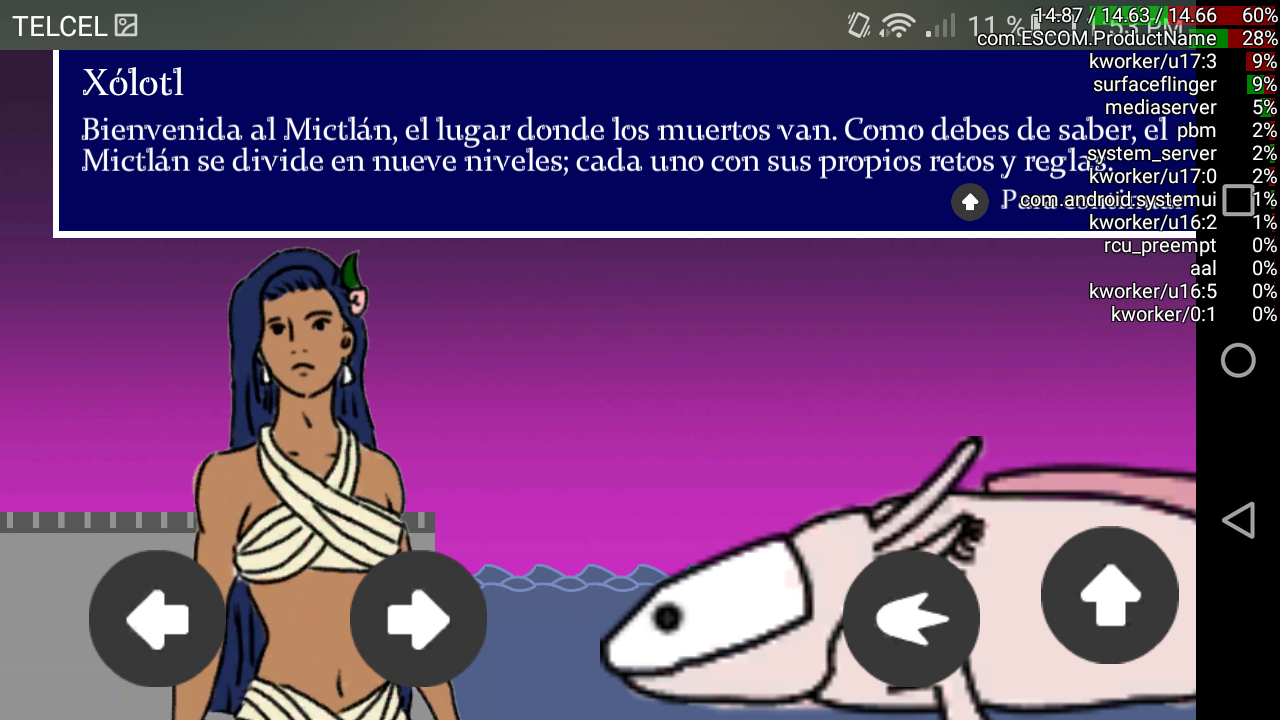
\includegraphics[width=0.4 \textwidth]{04ResultadosObetnidos/imagenes/rendimiento03.png}}
   
   \subfigure[Uso del GPU desde un nivel de plataforma.] {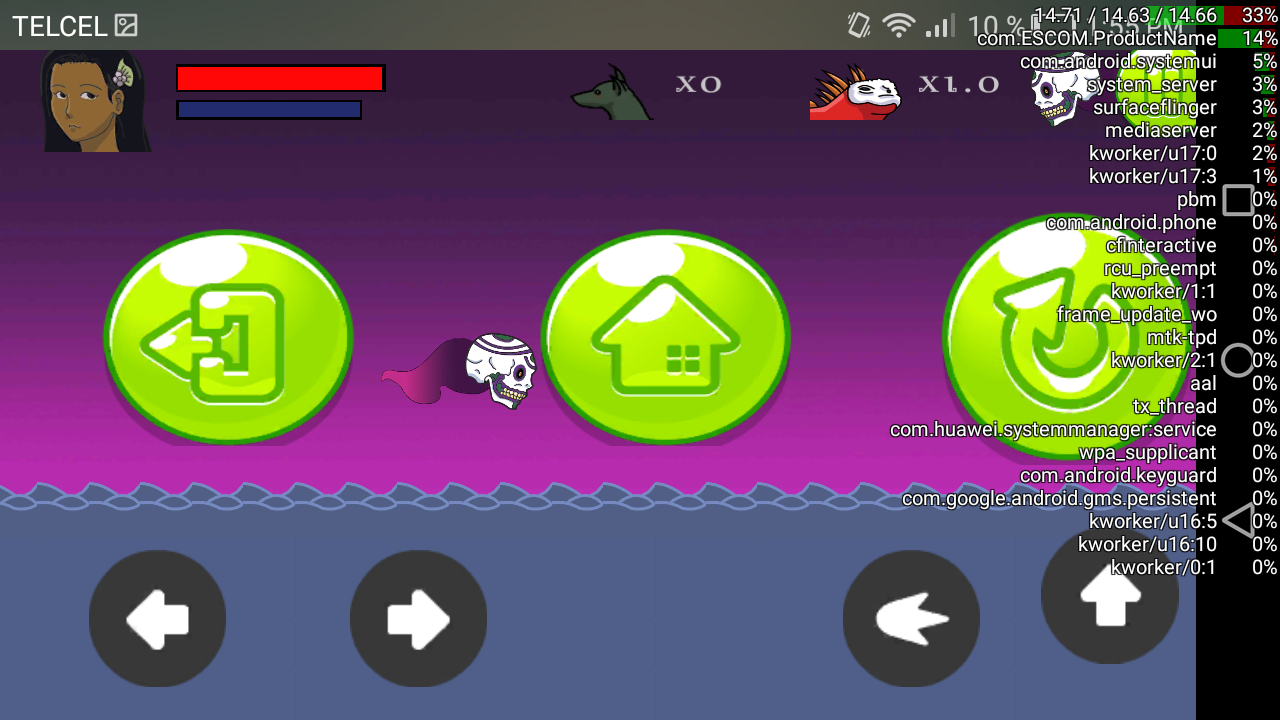
\includegraphics[width=0.4 \textwidth]{04ResultadosObetnidos/imagenes/rendimiento05.png}}
   
   \subfigure[Uso del GPU desde un nivel de jefe.] {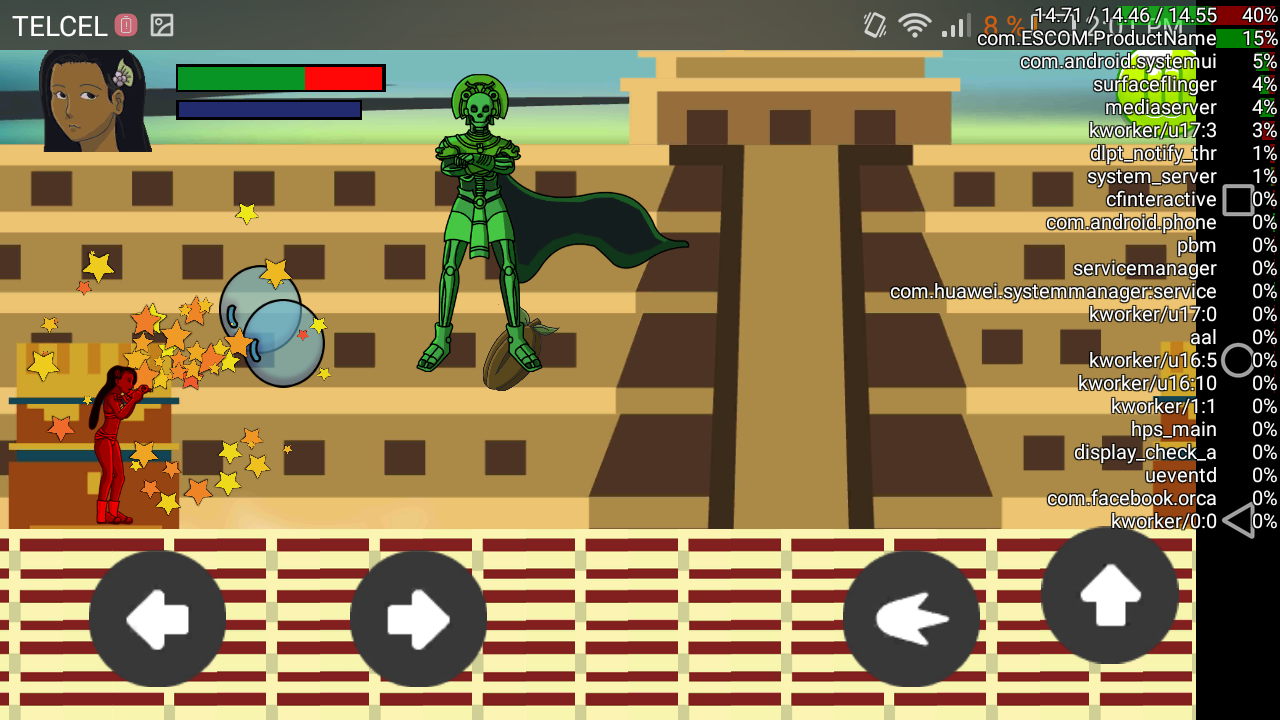
\includegraphics[width=0.4 \textwidth]{04ResultadosObetnidos/imagenes/rendimiento10.png}}
   
  \caption{Resultados del rendimiento del GPU del dispositivo Huawei}
  \label{fig:GPUHuawei}
\end{figure} 
                \begin{figure}[h]
                        \centering
                        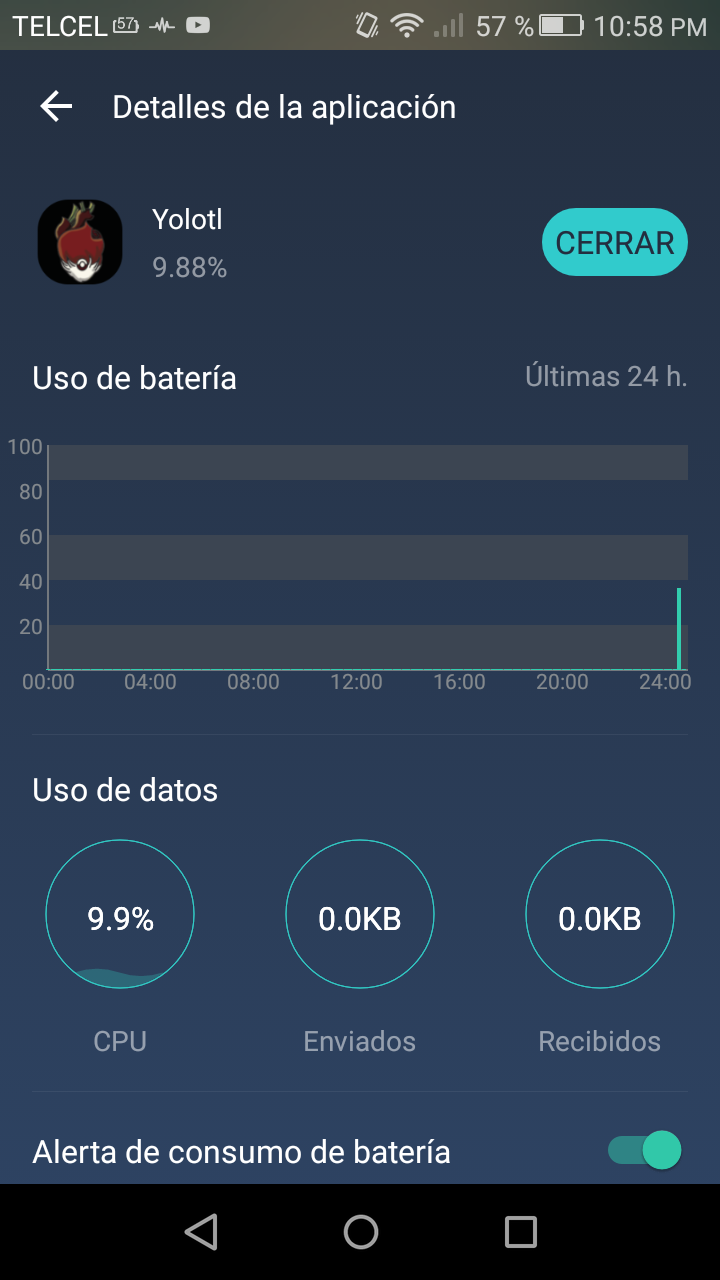
\includegraphics[width=0.2\textwidth]{04ResultadosObetnidos/imagenes/baterry02.png}
                        \caption{Pantalla de la aplicación \textit{Baterry Doctor} para medir el 
                        rendimiento del juego.}
                        \label{fig:BateriaYolotl}
                \end{figure}
\subsubsection{Conclusiones de la prueba}
De esta medición del desempeño del GPU se puede observar que la aplicación 
utiliza un mínimo del 9\% del GPU y hasta un máximo del casi el 30\%. Por su 
parte, el juego utiliza en promedio un 40\% de la batería. Estas cifras son 
buenas si se considera que otras aplicaciones como \textit{Messenger} de 
\textit{Facebook} llega a utilizar el 50.6\% del GPU y casi el 60\% de la batería 
del teléfono, ver figura \ref{fig:BateriaFacebook}. 
\begin{figure}[h]
                        \centering
                        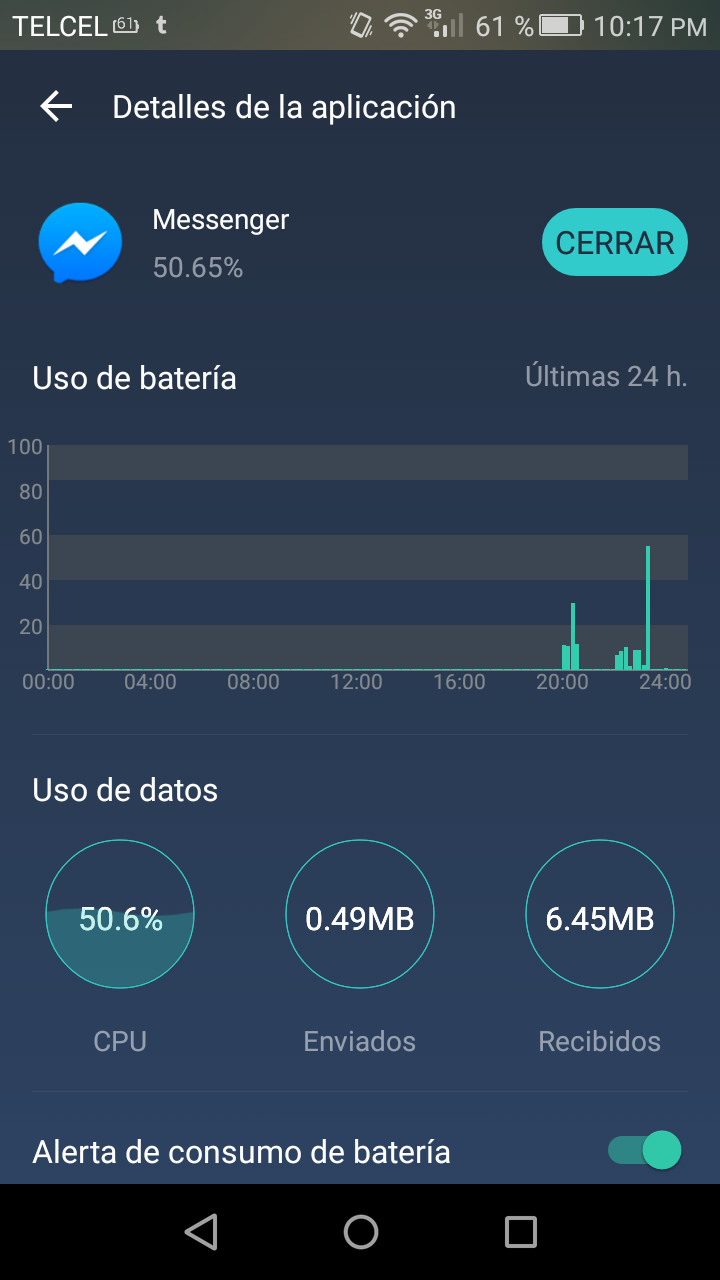
\includegraphics[width=0.2\textwidth]{04ResultadosObetnidos/imagenes/baterry01.png}
                        \caption{Pantalla de la aplicación \textit{Baterry Doctor} para medir el 
                        rendimiento de \textit{Messenger} de \textit{Facebook}.}
                        \label{fig:BateriaFacebook}
                \end{figure}

\subsection{Prueba de aceptación} \label{Cuestionario}
Esta prueba está basada en modelo de pruebas \textit{Game Flow}\cite{gameflow}.
\textit{Game Flow} utiliza estrategias heurísticas de usabilidad y experiencia
de usuario para medir el nivel de aceptación de los usuarios. Este modelo permite
medir varios aspectos de los cuales en este proyecto se probarán:
{\it enjoyment}(disfrute), diseño de interfaces, mecánicas y jugabilidad.
\\
\par
Se toma la decisión de aplicar las pruebas \textit{Game Flow} por nivel ya que en
caso de realizar modificaciones para mejorar la experiencia de usuario estos
cambios se podrán orientar a un nivel en especifico si al final de las pruebas
un nivel en específico genera problemas entre los usuarios por su elevada
dificultad o facilidad. Por otra parte aplicar las pruebas por niveles permite que los jugadores no tengan que jugar todo el videojuego para tener que responder la encuesta lo que traduce en que las pruebas no tomarán mucho del tiempo de los participantes.
\\
\par
Esta prueba de aceptación se dividió en dos partes:
\begin{itemize}
    \item \textbf{Presencial}: Esta prueba se realiza sobre la población de la
    Escuela Superior de Cómputo(ESCOM) del Instituto Politécnico Nacional(IPN).   
    \item \textbf{En línea:} Para esta prueba se publicaron los \textit{links} del
    archivo APK y de la encuesta en foros de desarrollo de videojuegos y grupos
    de \textit{FaceBook} con la misma temática.
\end{itemize}
 
\subsubsection{Objetivo}
Evaluar el nivel de aceptación de juego entre los jugadores y obtener la opinión
de los mismos sobre posibles mejoras al juego.

\subsubsection{Herramientas}
Para aplicar ambos tipos de pruebas se utilizaron:
    \begin{itemize}
        \item \textbf{Archivo APK del juego:} Este archivo fue proporcionado por
        medio de un \textit{link} y por medio de transferencia de archivos al teléfono
        de los encuestados desde una computadora.
        \item \textbf{Cuestionario:} El cuestionario fue proporcionado desde un
        \textit{link} empleando la herramienta de \textit{Google Docs} para agilizar
        el conteo de los resultados.   
    \end{itemize}

\subsubsection{Aplicación}
Para la aplicación de las pruebas en línea se distribuyen los links del archivo APK y del cuestionario en diferentes foros de desarrolladores y grupos de \textit{Facebook}. En algunos casos diferentes usuarios ofrecieron retroalimentación del juego en los comentarios de la publicación o enviando mensajes privados.
\\
\par
En el caso de las pruebas presenciales, se solicita a diferentes profesores del
plantel de la ESCOM. En cada uno de los grupos en los que se aplica la encuesta
se da una presentación del argumento del juego y su objetivo. Después se dan las
instrucciones de la prueba, los \textit{link} a los archivos y al cuestionario y
se indica el nivel a probar. Además de la encuesta se puede observar las
reacciones de lo jugadores mientras prueban el juego
(ver figura \ref{fig:AlumnosESCOM}).

\begin{figure}
  \centering
 
   \subfigure[Dos alumnos de la Escuela Superior de Cómputo probando el juego.] {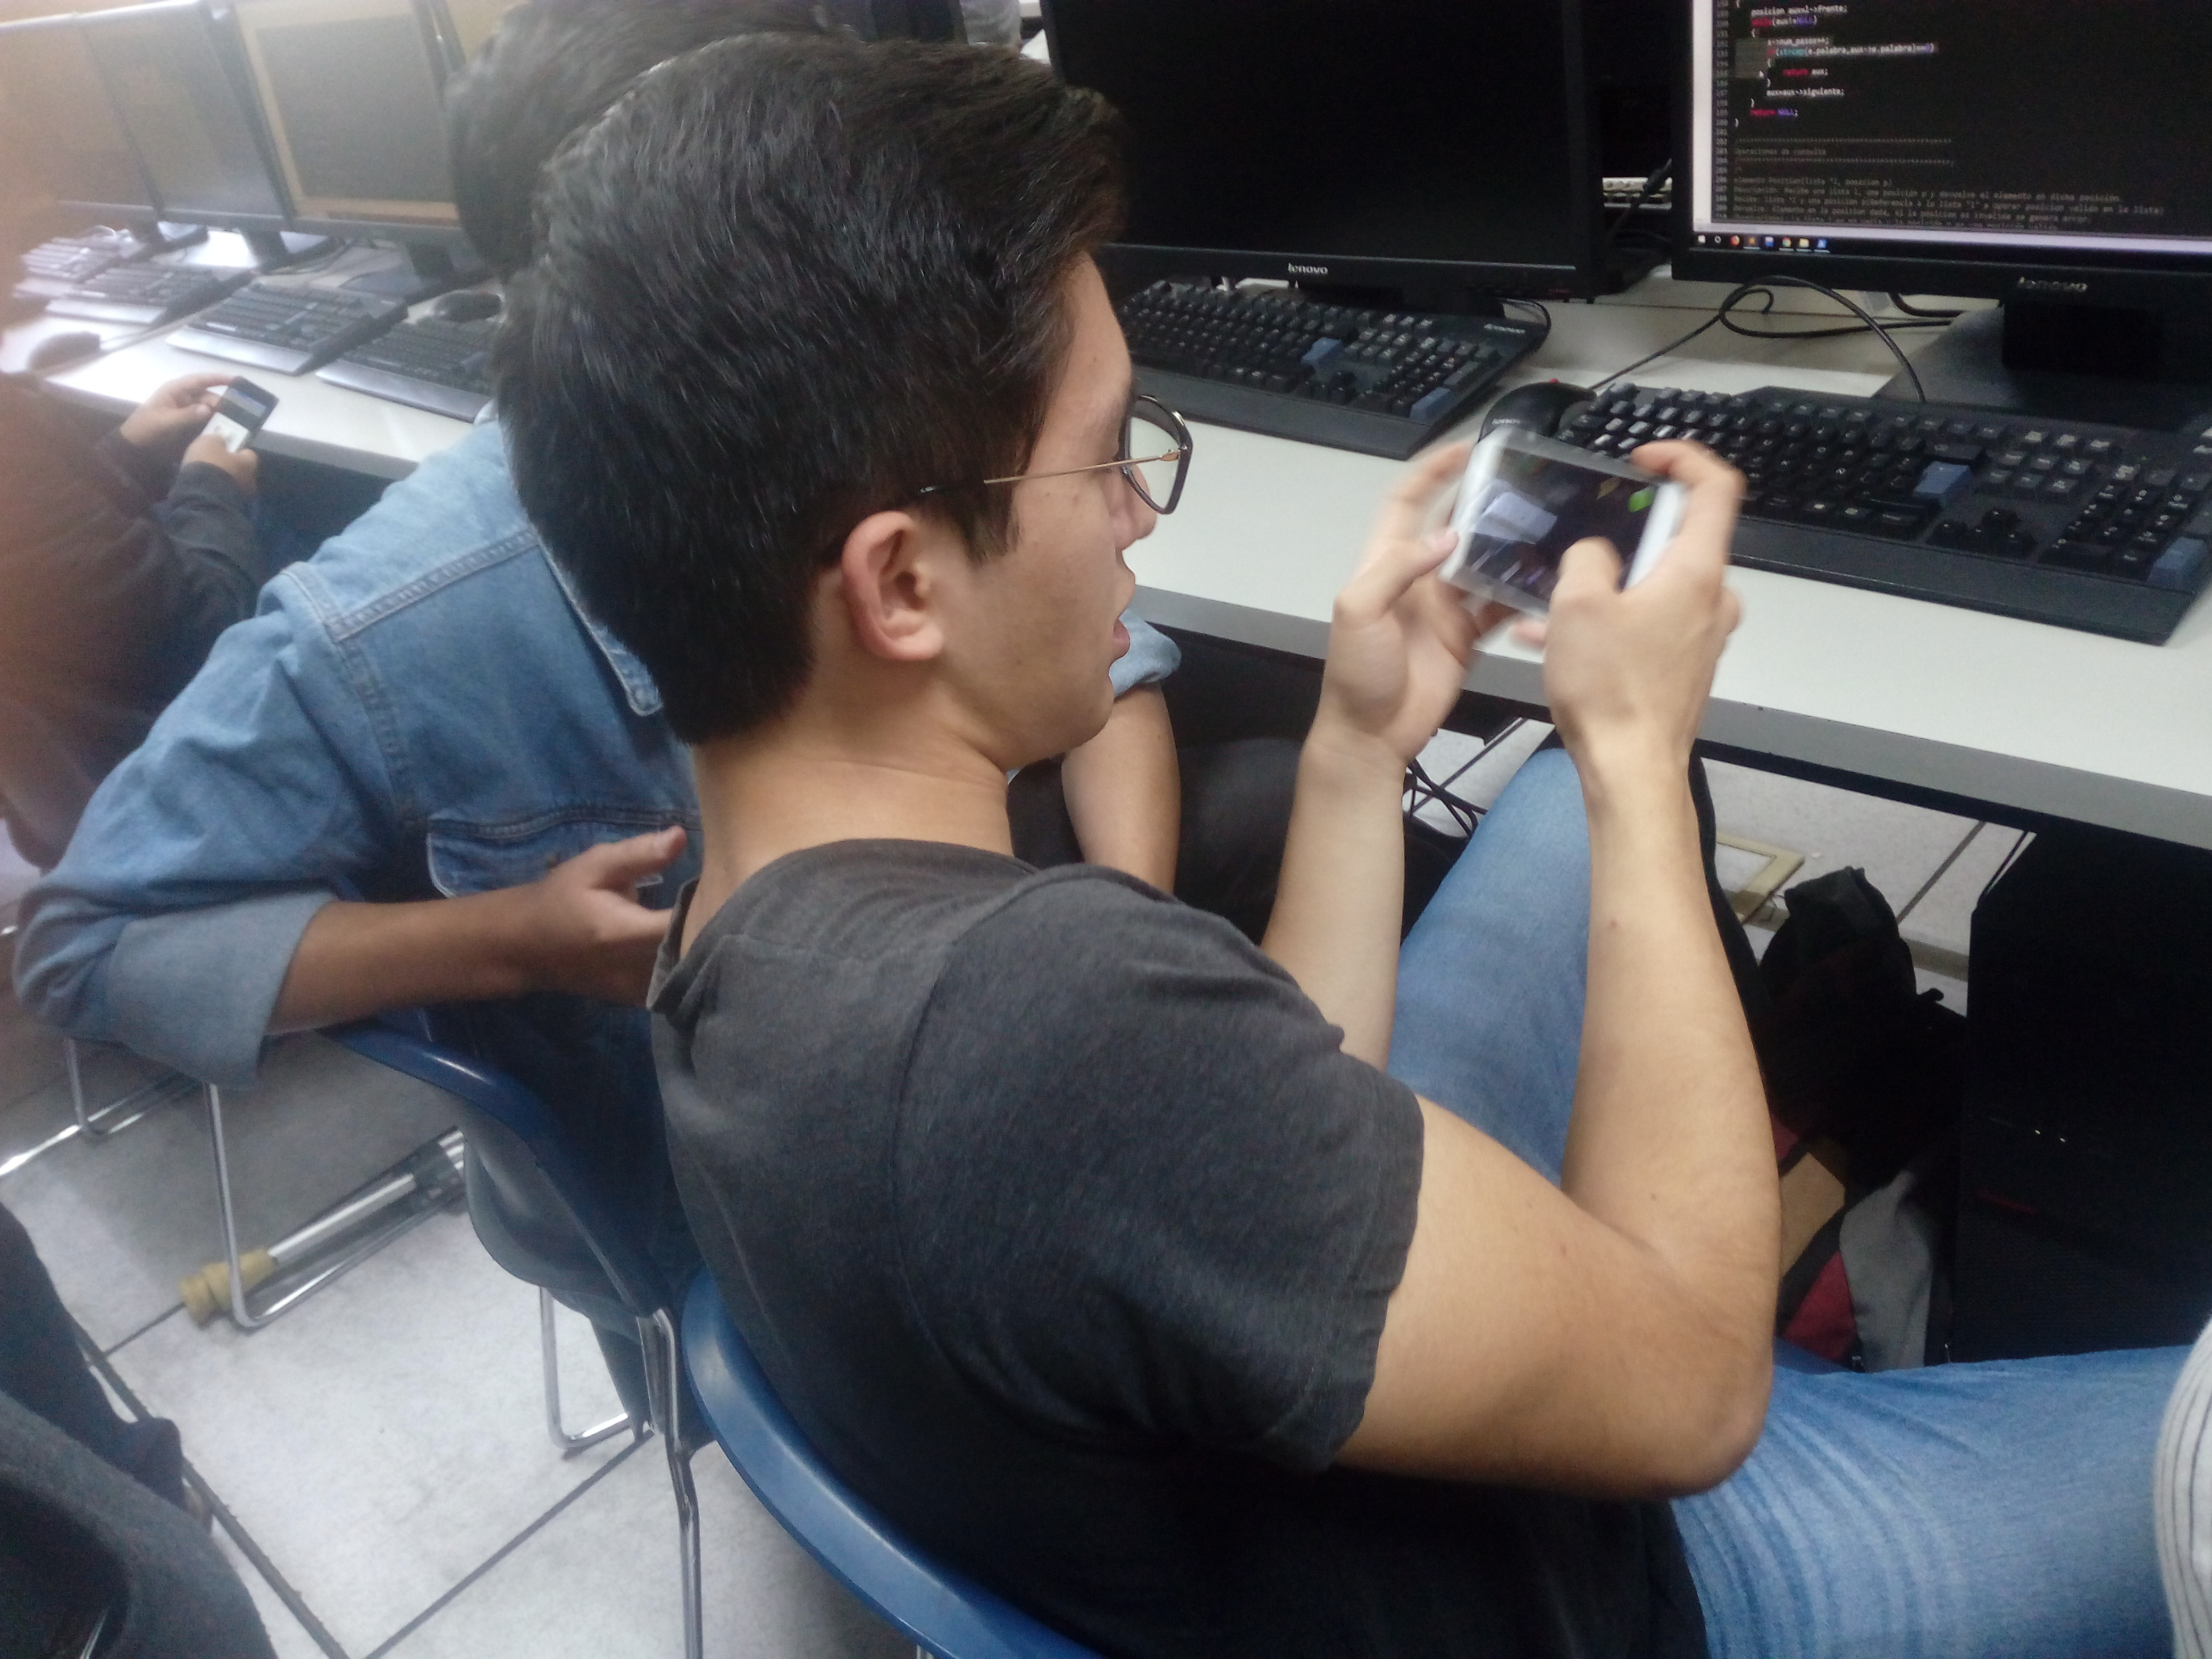
\includegraphics[width=0.4 \textwidth]
   {04ResultadosObetnidos/imagenes/usuarios01}}
        
        \subfigure[Grupo de alumnos de la Escuela Superior de Cómputo probando el
        juego.] {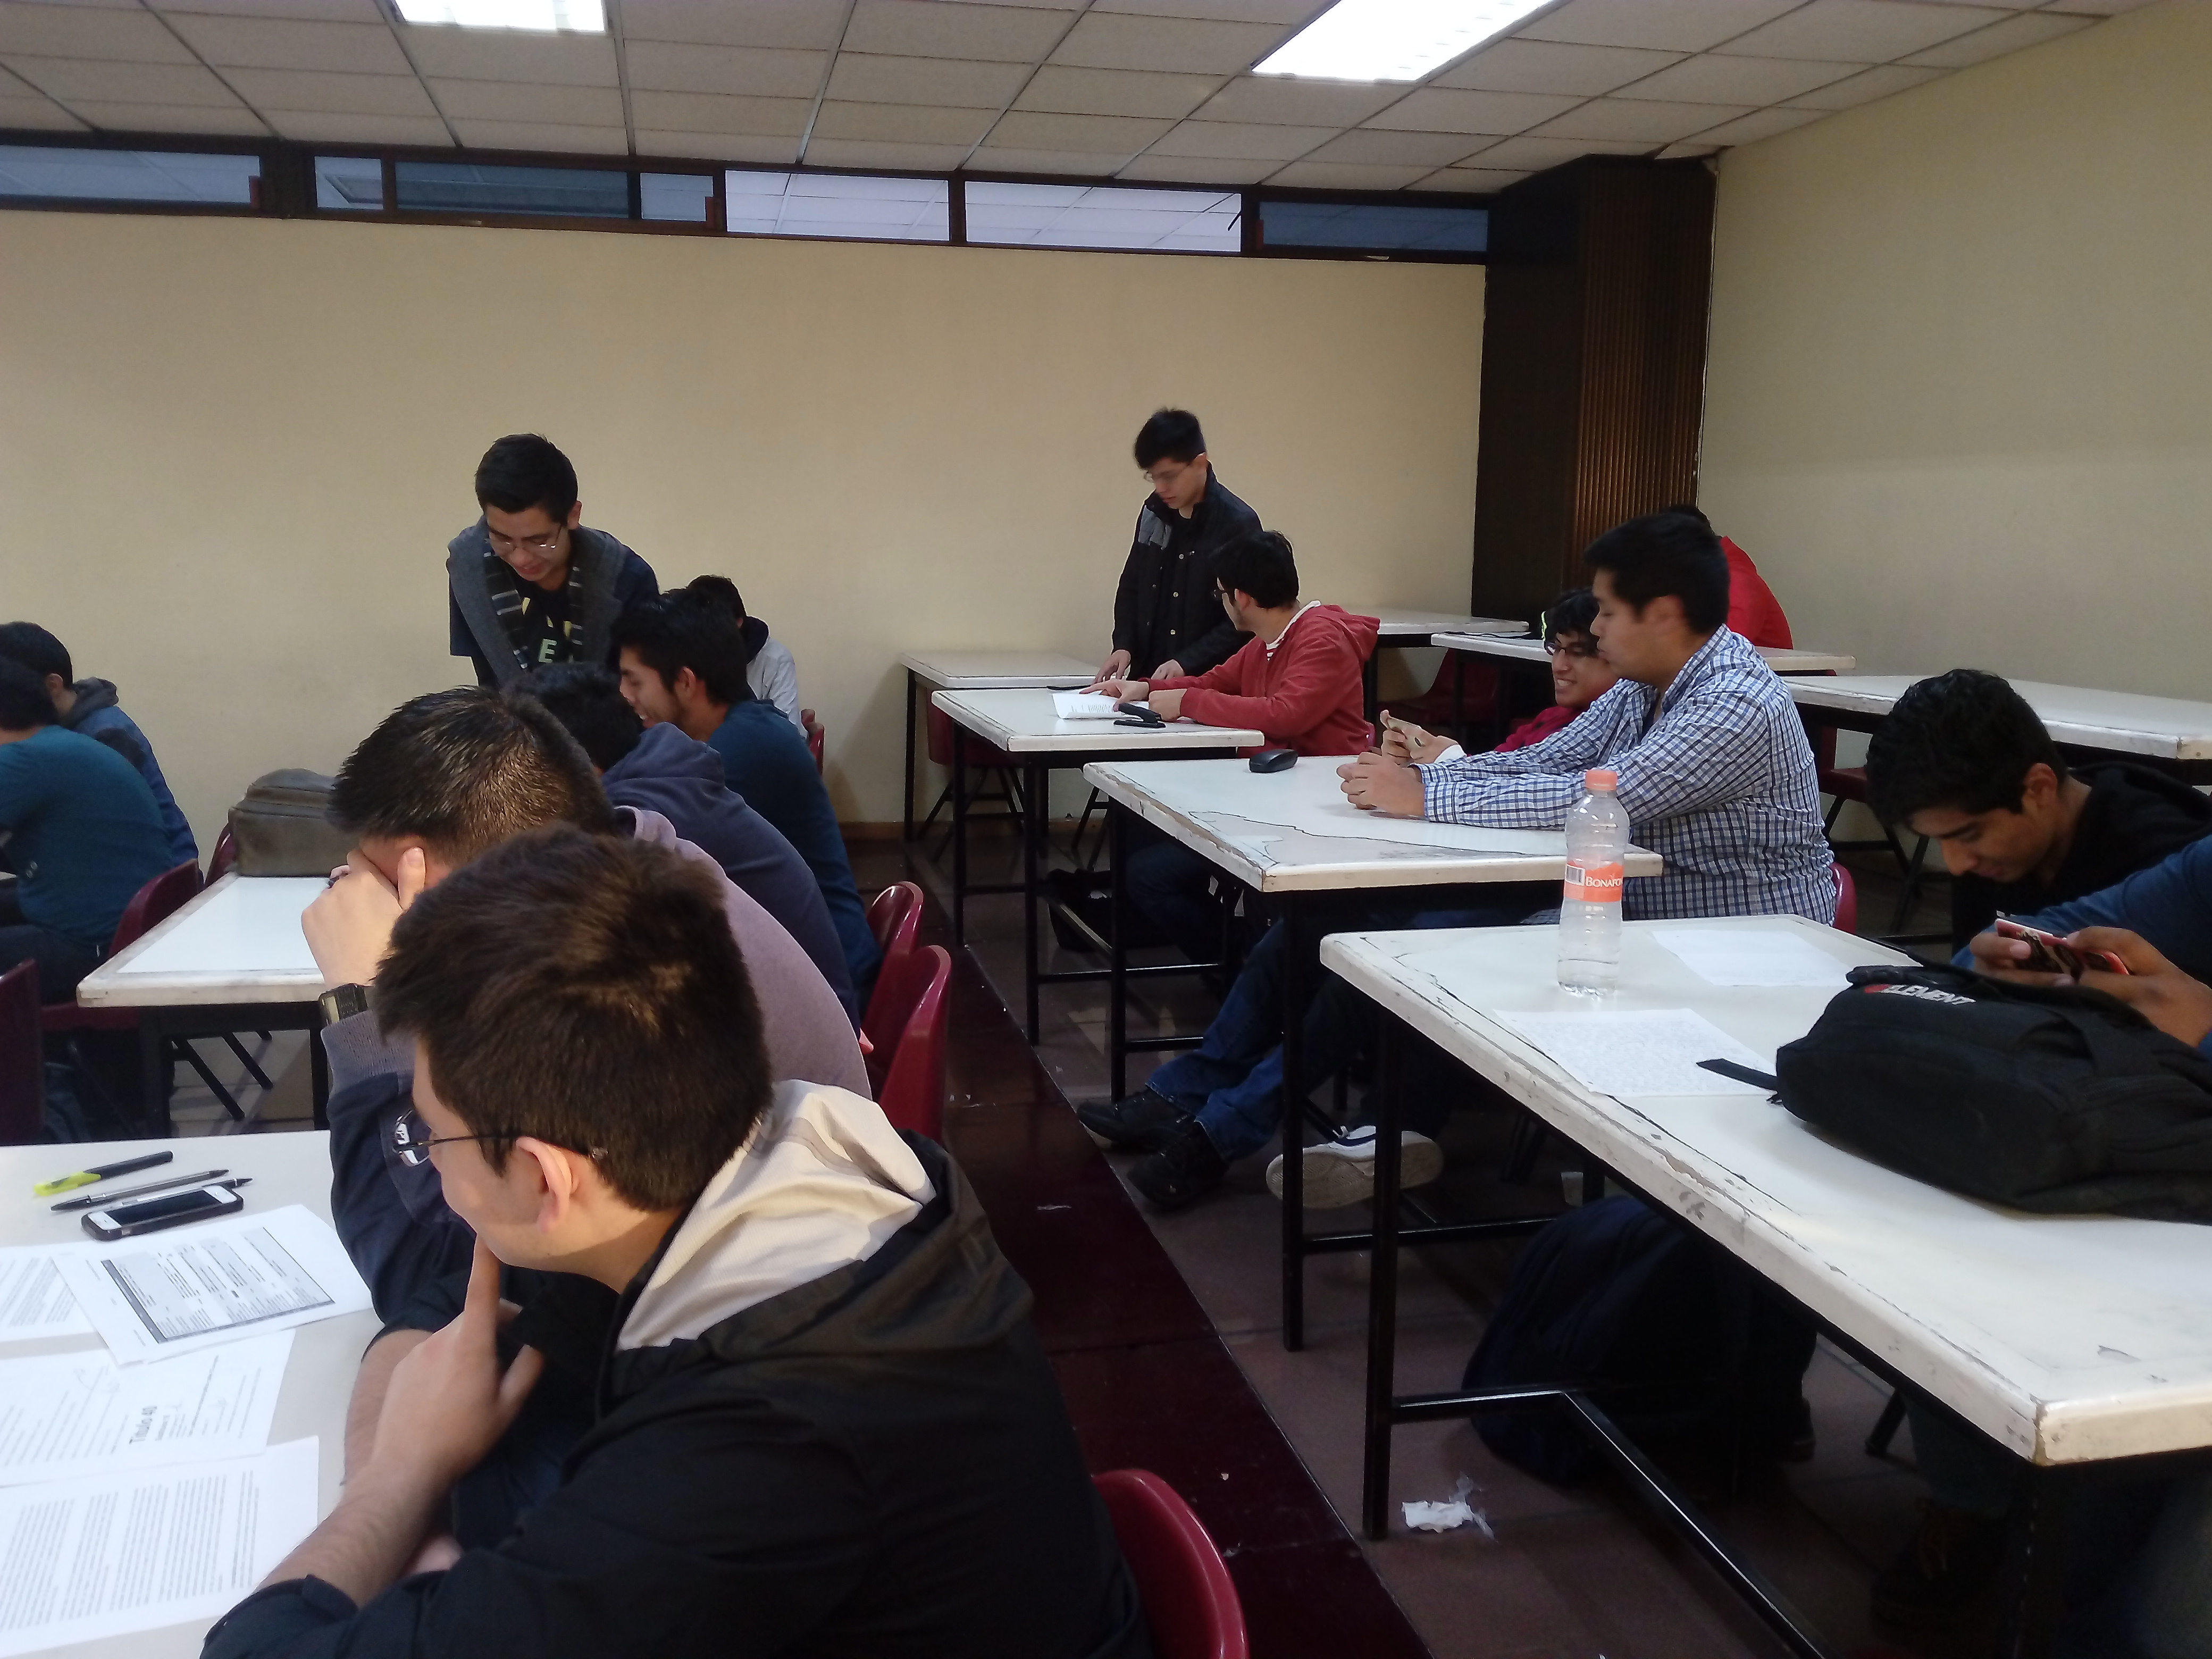
\includegraphics[width=0.4 \textwidth]{04ResultadosObetnidos/imagenes/usuarios02}}
  \caption{Resultados de la herramienta \textit{profiler} al analizar una cinemática.}
  \label{fig:AlumnosESCOM}
\end{figure}

\subsubsection{Resultados}
A continuación se presentan algunos de los resultados de la encuesta,
lo resultados completos se encuentran en el anexo \ref{Anexo:resultados}.
\begin{itemize}
        \item La principal marca de dispositivos con el que fue probado el juego fue
        Motorola con sistema operativo Android 7.
        \item La mayoría de los usuarios consideran como bueno el movimiento del
        personaje.
        \item La mayoría de los usuarios consideran que la respuesta de la
        \textit{GUI} es buena.
        \item La mayoría de los usuarios opina que la actualización de la barra de
        tonali es buena pero les gustaría que existiera un indicador numérico para ver
        la cantidad de disparos que les queda.
        \item La mayoría de los usuarios considera que lo hace hace débil a un personaje
        es su patrón de movimiento y no la cantidad de daño que pueda generar; por
        otro lado también la mayoría de los usuarios considera que lo que hace a un
        enemigo fuerte es su patrón de movimiento.
        \item El Fantasma morado es considerado por muchos usuarios como el enemigo más
        poderoso en los niveles de plataforma.
        \item El fantasma rojo es considerado por muchos usuarios como el enemigo más
        débil en los niveles de plataforma.
        \item Las dos principales causas de muerte en los jugadores son el tiempo
        de respuesta de la \textit{GUI} y que los enemigos eran demasiado fuertes.
\end{itemize}

Adicionalmente lo jugadores hicieron observaciones y peticiones que ellos
consideran podrían mejorar la experiencia de juego:
\begin{itemize}
        \item Animación que indique que un enemigo ha recibido daño.
        \item Barra de vida para los enemigos.
        \item Posibilidad de que el jugador se agache.
        \item Mensajes de confirmación para los botones que llevan al menú de selección
        y que cierran la aplicación.
        \item Mejorar el comportamiento de los disparos.
\end{itemize}

\subsubsection{Conclusiones}
Las conclusiones que se obtuvieron de las pruebas son:
    \begin{itemize}
        \item Hacer el salto más estable mejorará la experiencia del jugador.
        \item Mejorar el tiempo de respuesta de la GUI y agregar una animación
        que indique que un botón ha sido oprimido mejorará la experiencia del
        jugador ya que la mayoría de los usuarios indica que este aspecto fue la
        causa de la mayoría de sus muertes dentro del juego.
        \item Si se desea hacer niveles de plataforma más difíciles estos deben
        de contener más enemigos normales de tipo Fantasma Morado ya que estos son
        los que la mayoría de los jugadores consideran como el más fuerte.
        \item Si se desea hacer niveles de plataforma más fáciles estos deben
        de contener más enemigos normales de tipo Fantasma Rojo ya que estos son los
        que la mayoría de los jugadores consideran como el más débil.
    \end{itemize}

%\subsection{Cuestionario 4}

\subsubsection{Pre-juego}
	
	 ¿Cuál es tu edad? \\
	Respuesta: El público en su mayoría que ha respondido la encuesta se encuentra entre los 21 y 25 años de edad y algunas personas entre los 30 y 40 años. \\ 
	
	 ¿Cuál es tú nivel de estudios? \\
	\begin{itemize}
		\item Básica
		\item Media superior
		\item Superior
		\item Doctorado o maestría
	\end{itemize}

\begin{figure}
	\centering
	\caption{Gráfica de nivel de estudios}
	\label{fig:pre01}
	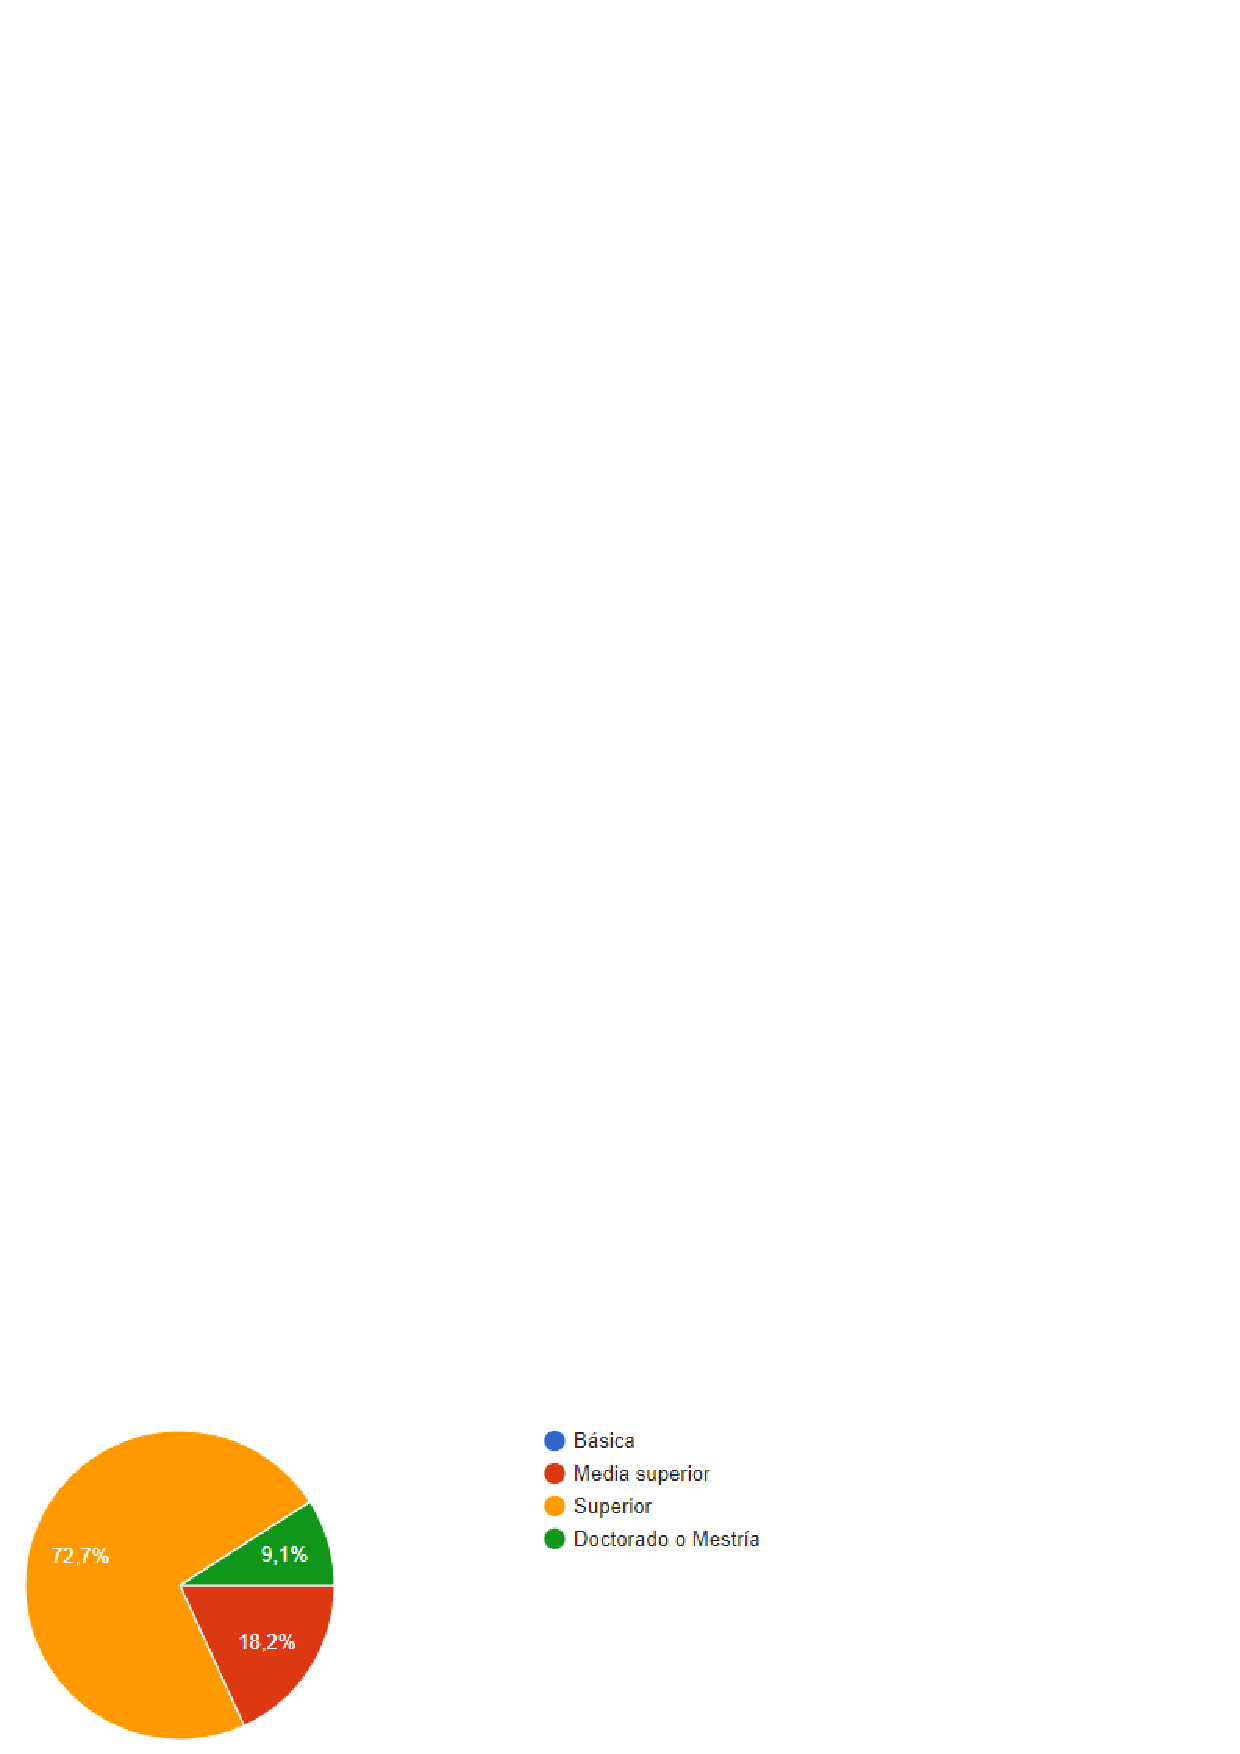
\includegraphics[width=0.5\textwidth]{04ResultadosObetnidos/pruebaR/imagenes/que/pre01}
\end{figure}

	
	 ¿Qué es lo primero que piensas cuando te dicen "cultura de México"?
	\begin{itemize}
		\item Comida
		\item Arquitectura o lugares
		\item Vestimenta
		\item Música
		\item Idioma	
	\end{itemize}

\begin{figure}
	\centering
	\caption{Gráfica de cultura de México}
	\label{fig:pre02}
	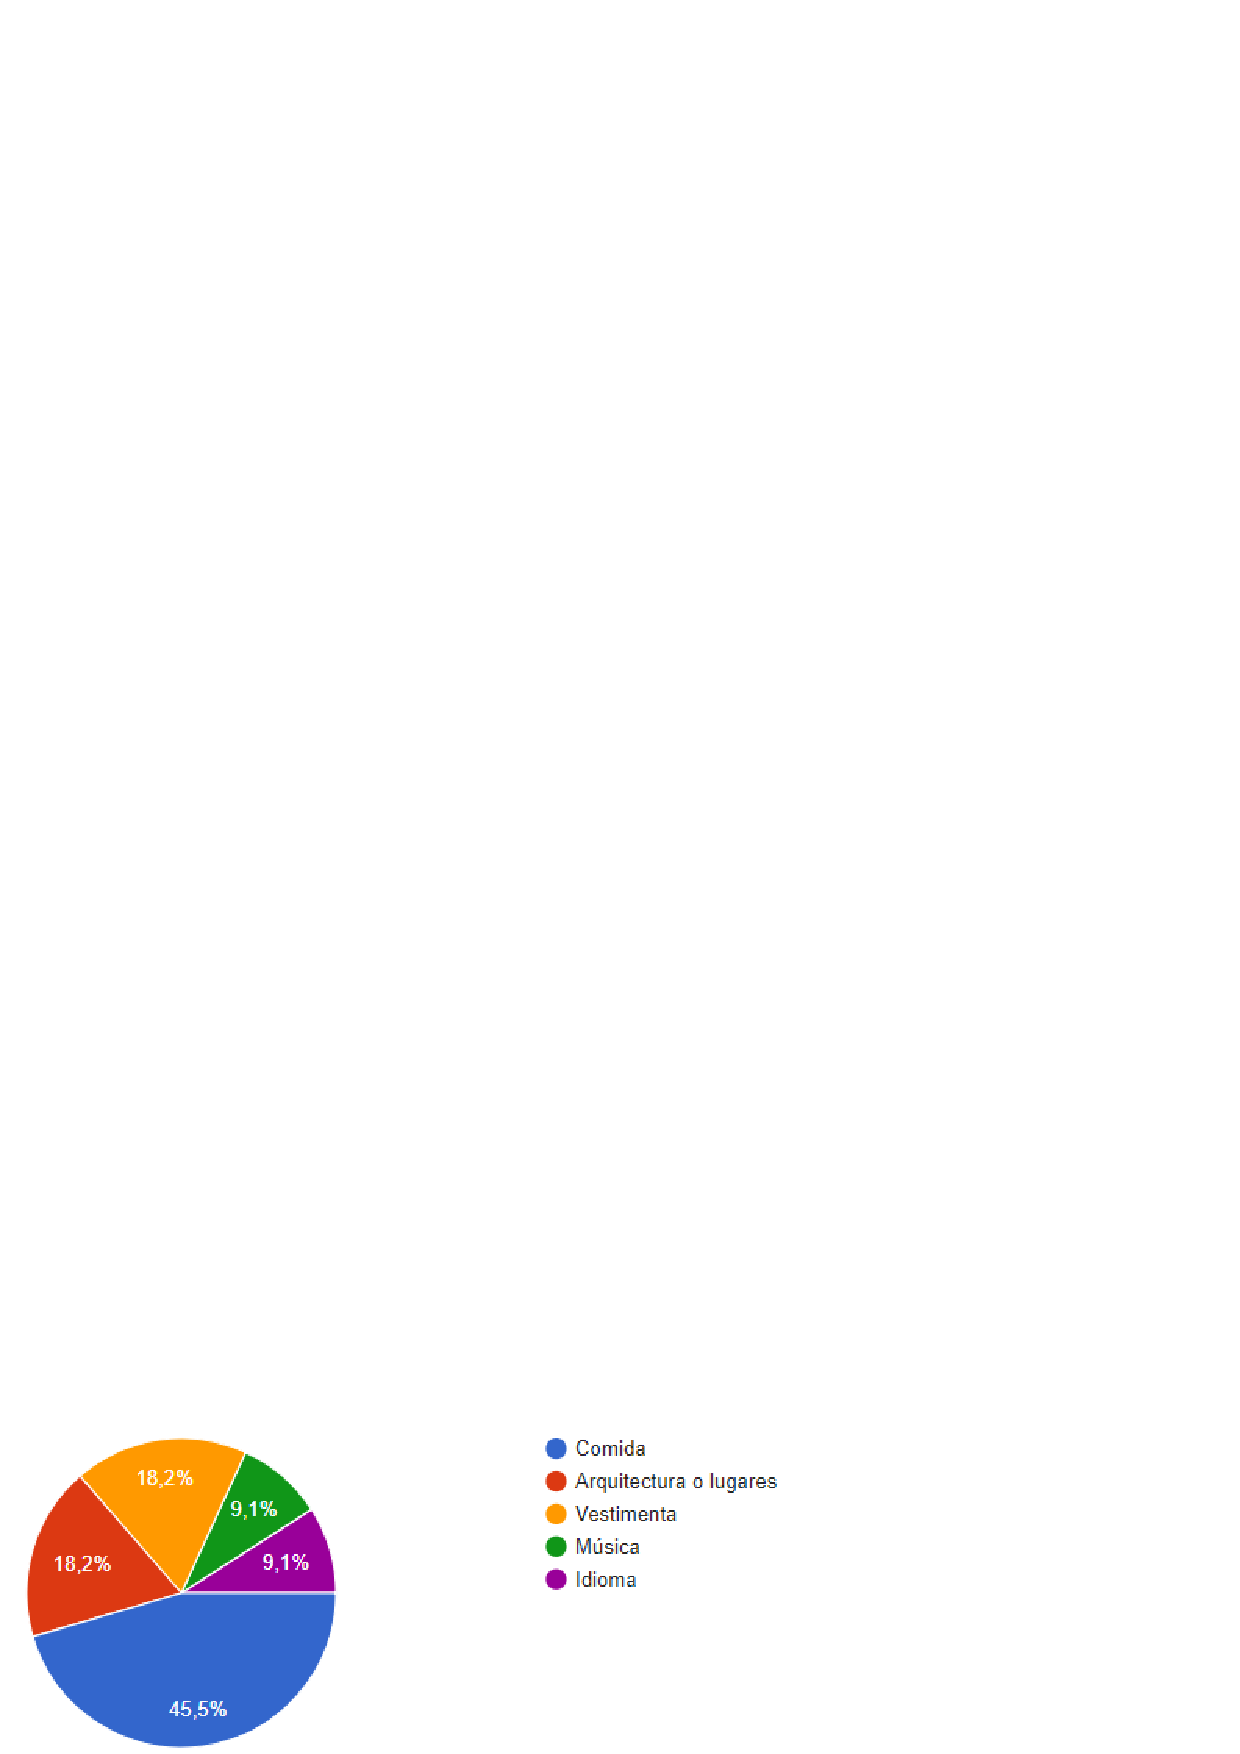
\includegraphics[width=0.5\textwidth]{04ResultadosObetnidos/pruebaR/imagenes/que/pre02}
\end{figure}

	
	¿Por qué motivos visitas lugares históricos?
	\begin{itemize}
		\item Escuela
		\item Trabajo
		\item Evento especial
		\item Interés propio
		\item Otro?
	\end{itemize}

\begin{figure}
	\centering
	\caption{Gráfica de lugares históricos}
	\label{fig:pre03}
	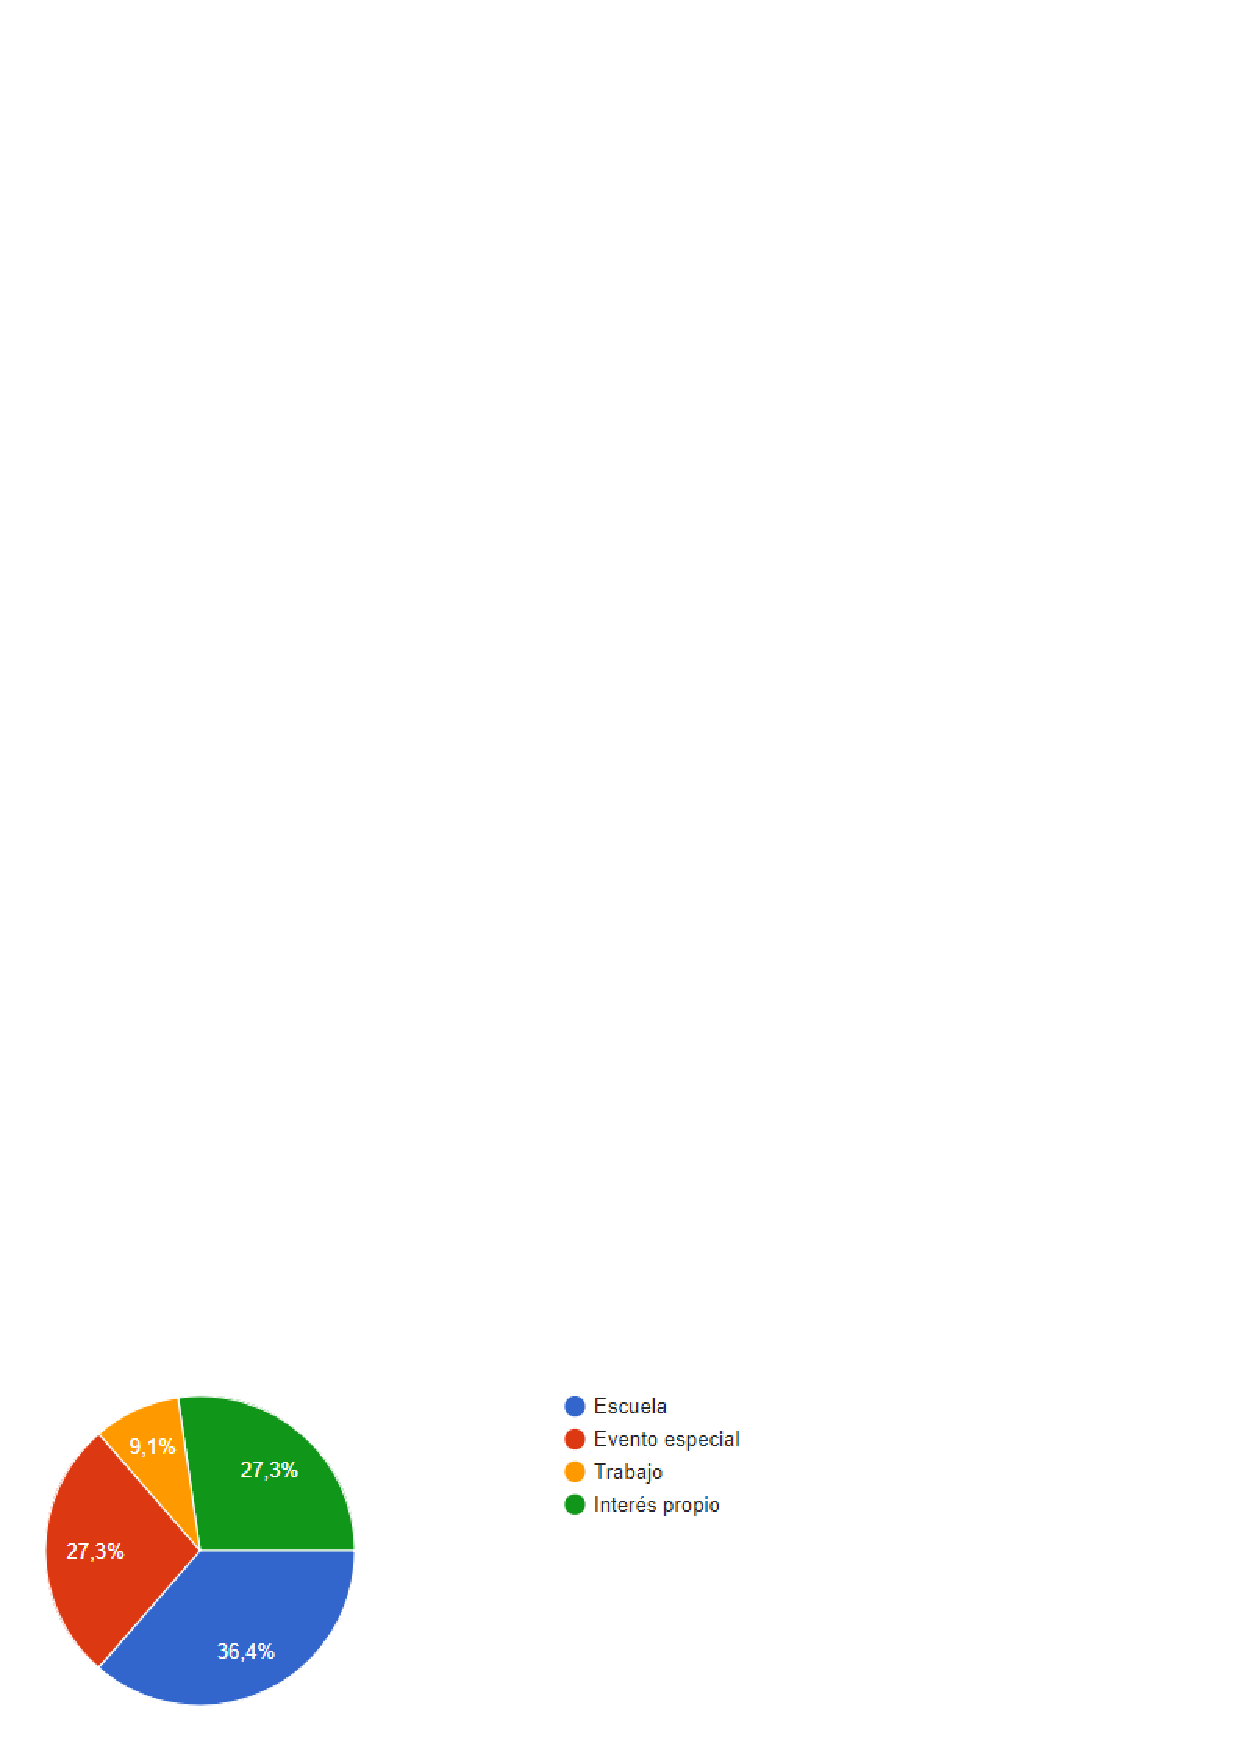
\includegraphics[width=0.5\textwidth]{04ResultadosObetnidos/pruebaR/imagenes/que/pre03}
\end{figure}

	
	¿Sabes sobre la cultura prehispánica en México?
	\begin{itemize}
		\item Sí
		\item No
		\item Creo
	\end{itemize}

\begin{figure}
	\centering
	\caption{Gráfica de cultura prehispánica}
	\label{fig:pre04}
	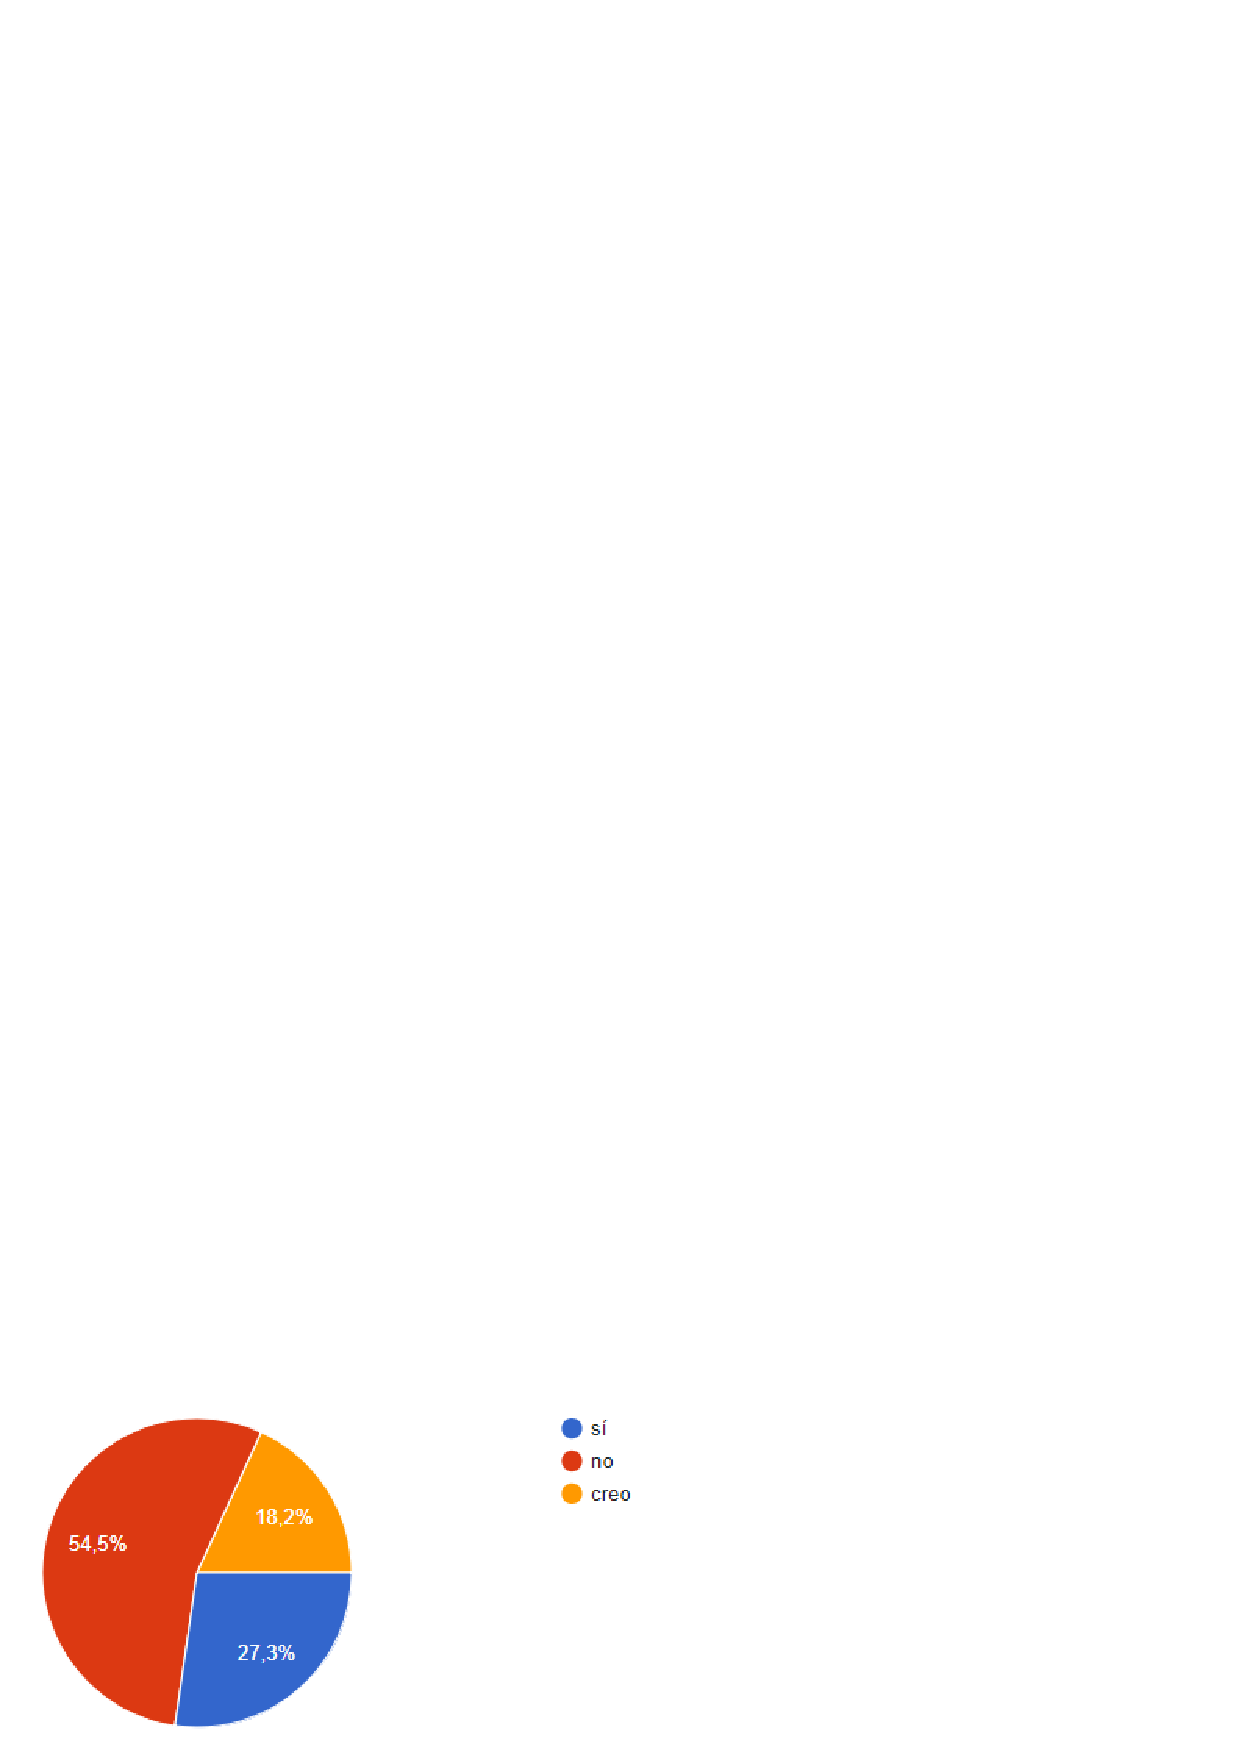
\includegraphics[width=0.5\textwidth]{04ResultadosObetnidos/pruebaR/imagenes/que/pre04}
\end{figure}

	
	¿Qué senitmiento tienes? 
	\begin{itemize}
		\item Alegría
		\item Enojo
		\item Tristeza
		\item Curiosidad
		\item Fatiga
		\item Otro?
	\end{itemize}

\begin{figure}
	\centering
	\caption{Gráfica de sentimiento}
	\label{fig:pre05}
	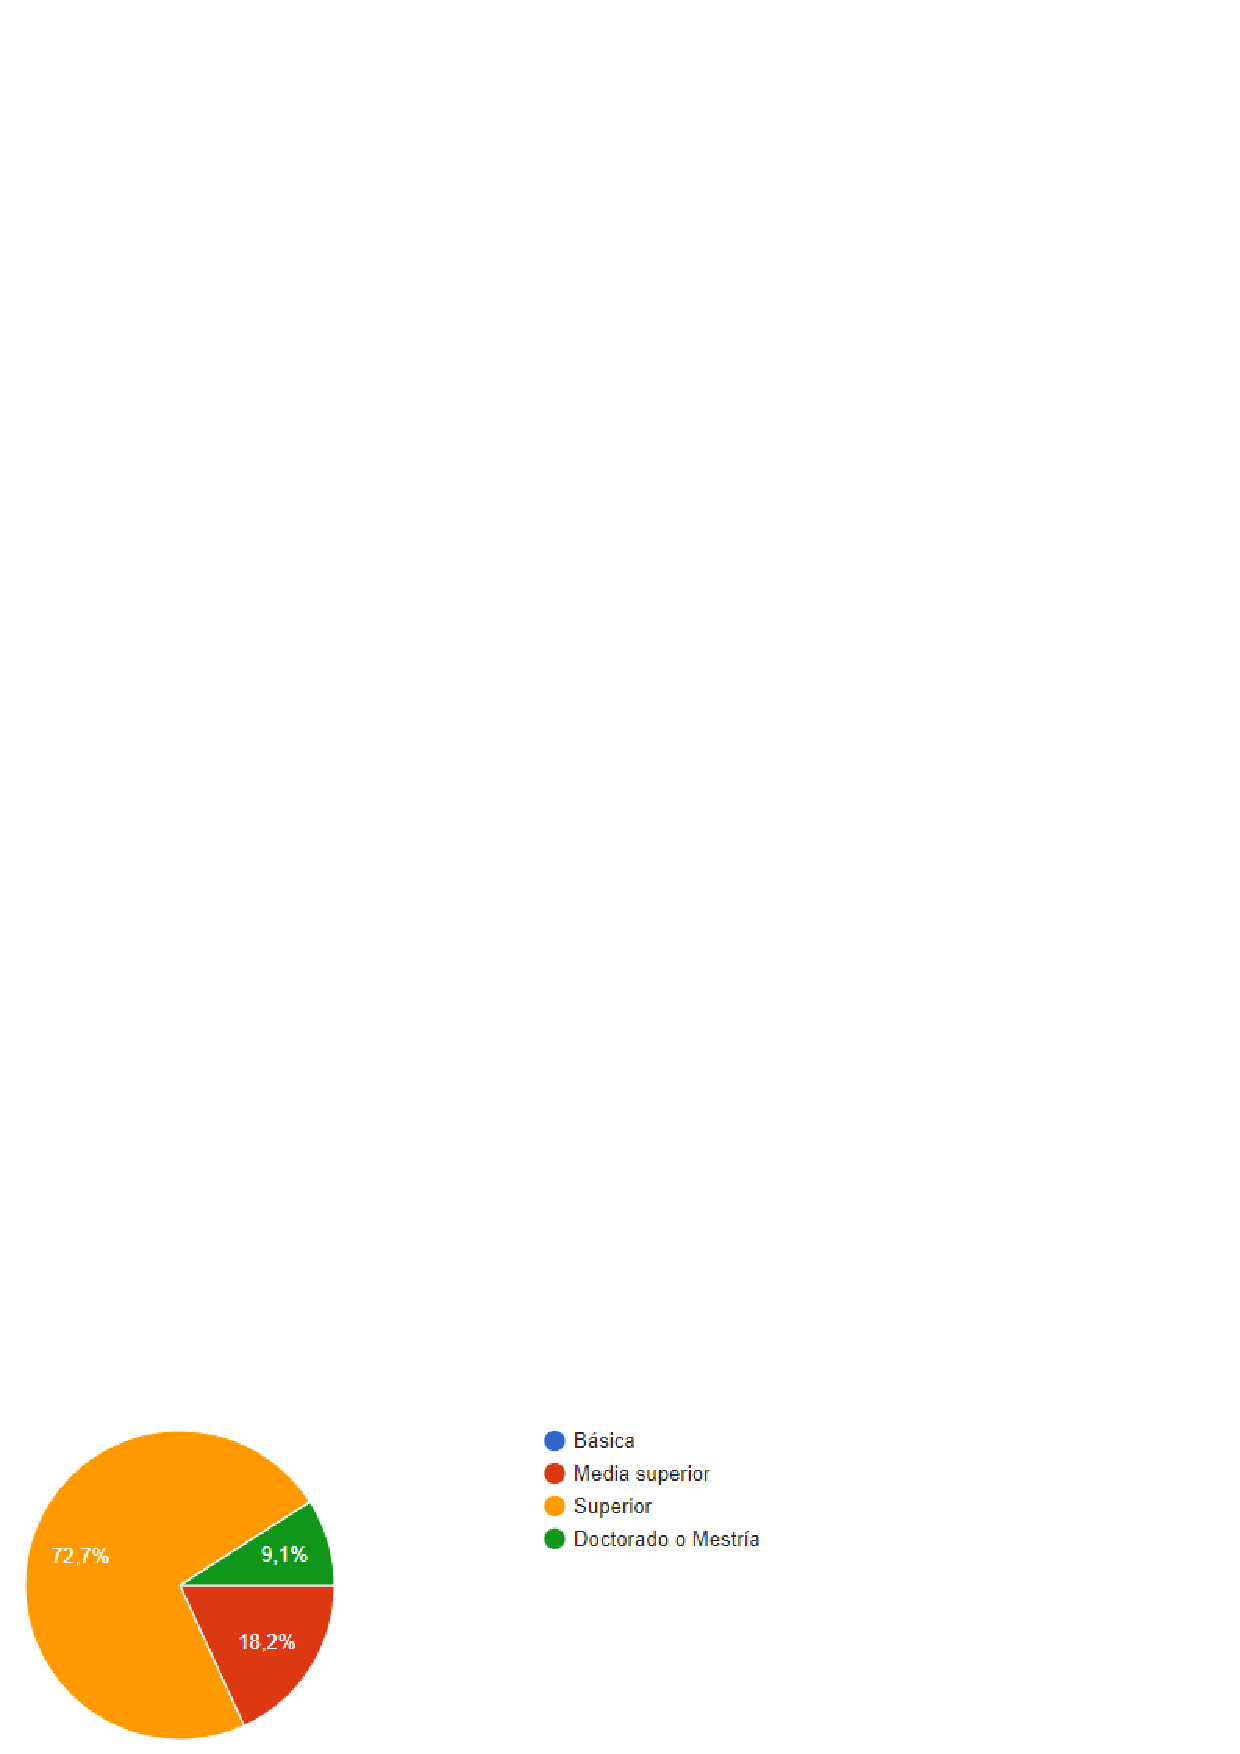
\includegraphics[width=0.5\textwidth]{04ResultadosObetnidos/pruebaR/imagenes/que/pre01}
\end{figure}

	
	 Pirámide emocional. ¿En que escalón te encuestras ahora?
	%%poner imagen
	La emoción que tenían los encuestados en ese momento era un estado de seguridad o tranquilidad.
	
	


\subsubsection{Post-juego}

	
 changing checkbox style locally
	¿Hay algún elemento que no reconozcas  o sepas que es?
	\begin{itemize}
		\item Items
		\item Personajes
		\item Fondo
		\item Texto (palabra)
		\item Lugar
		\item Tiempo
		\item Forma
		\item Otro?
	\end{itemize}

Respuesta: Los encuestados en su mayoría no reconocian diferentes formas o imágenes de objetos presentados en el juego.	

	¿Cómo califica la velocidad de reacción de los botones?
	\begin{itemize}
		\item Mala
		\item Regular
		\item Buena
	\end{itemize}

\begin{figure}
	\centering
	\caption{Gráfica de velocidad de botoness}
	\label{fig:pos01}
	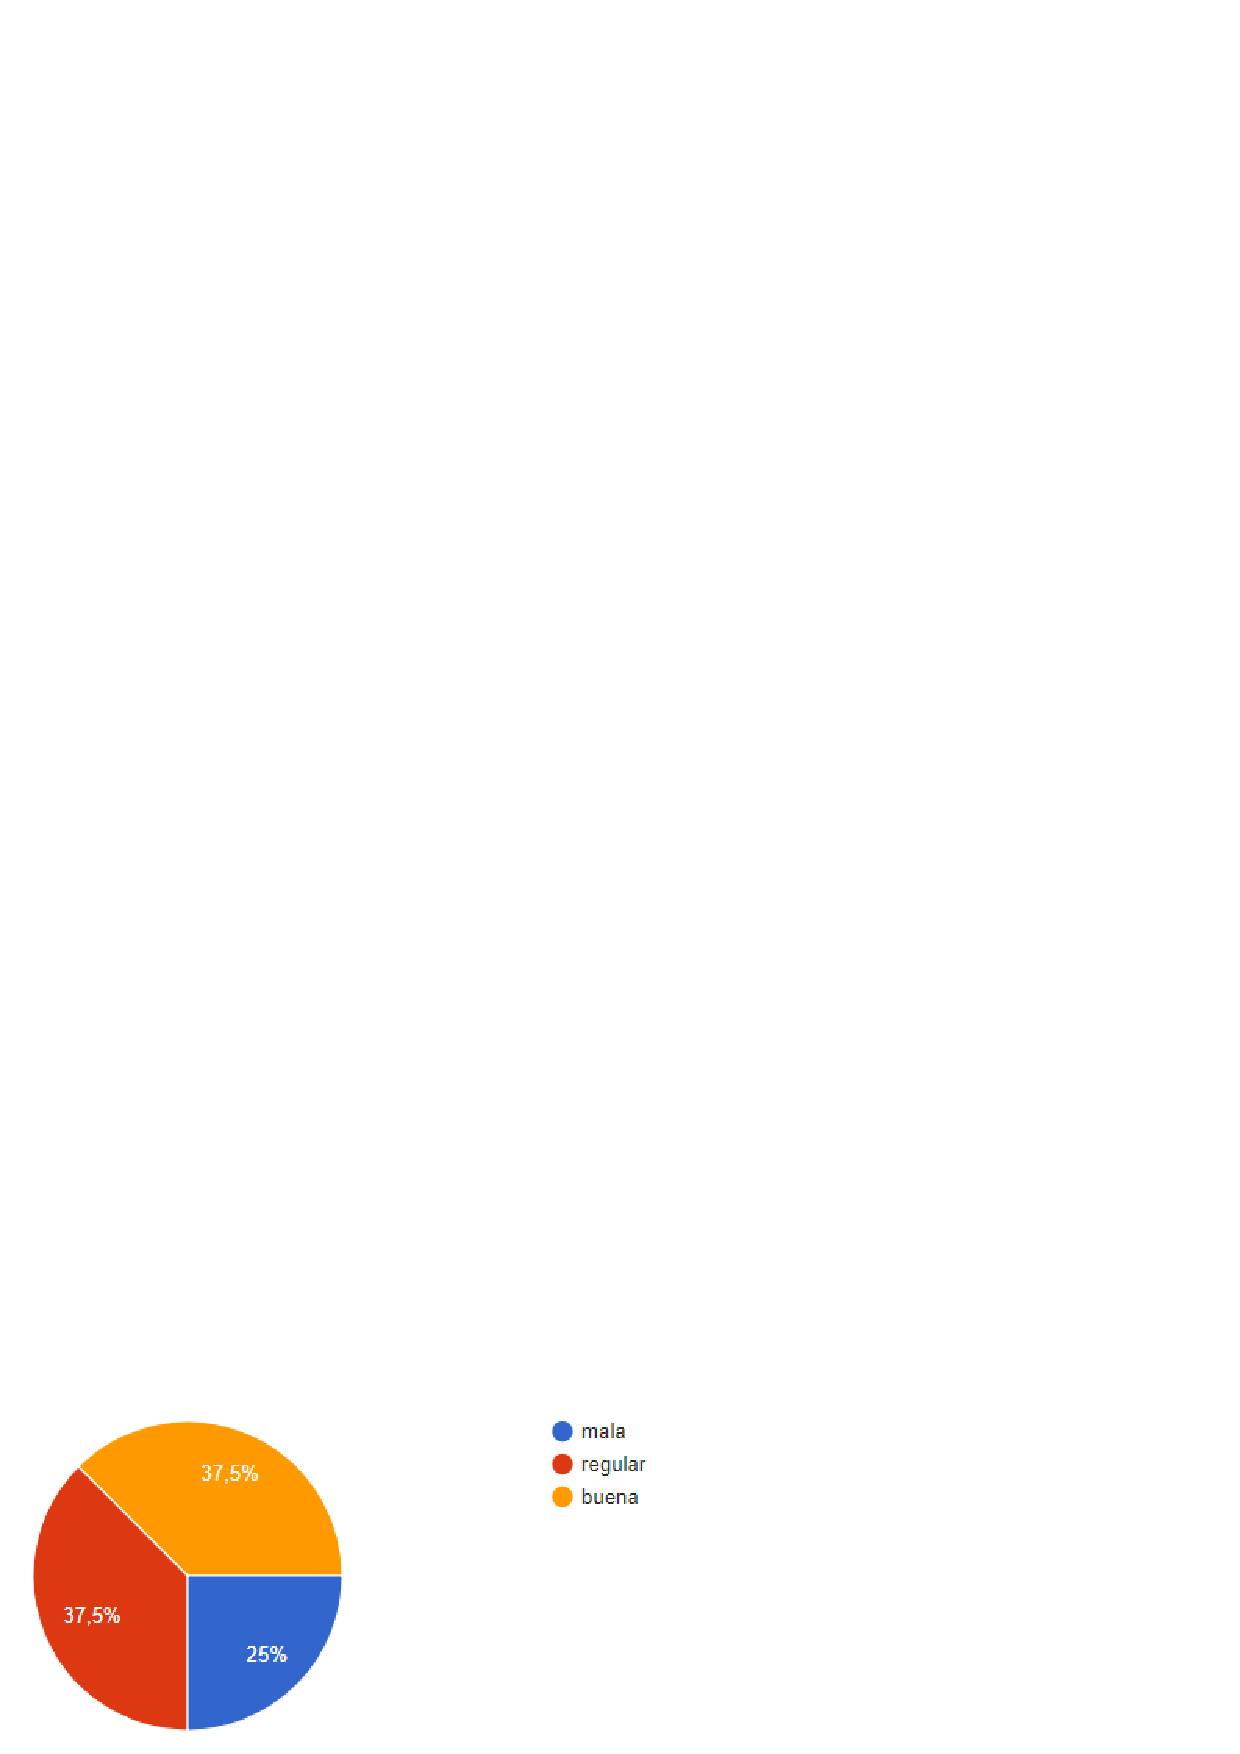
\includegraphics[width=0.5\textwidth]{04ResultadosObetnidos/pruebaR/imagenes/que/pos01}
\end{figure}

 ¿Qué te ha gustado MENOS del juego?
	\begin{itemize}
		\item Juego
		\item Dibujo
		\item Historia
		\item Temática
		\item Plataforma
	\end{itemize}

\begin{figure}
	\centering
	\caption{Gráfica de menos gusto}
	\label{fig:pos02}
	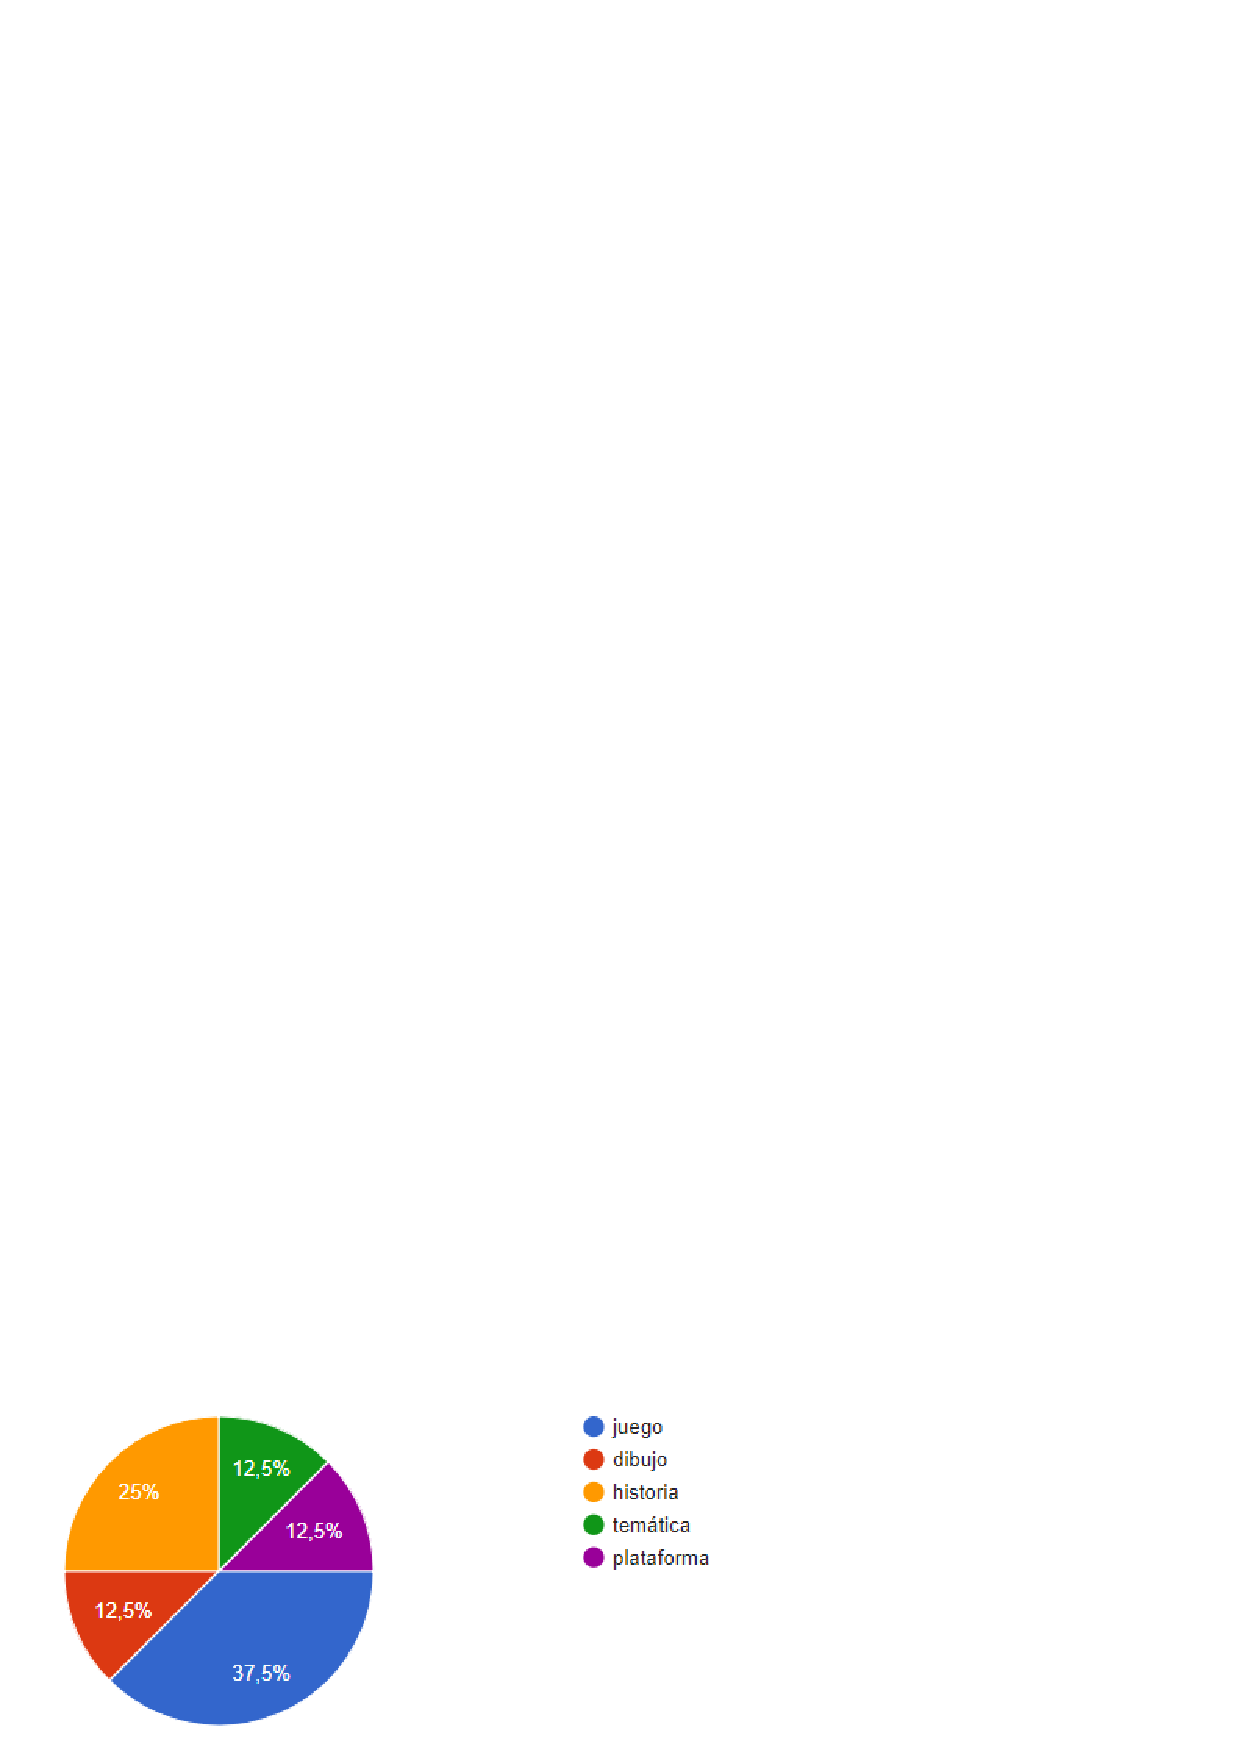
\includegraphics[width=0.5\textwidth]{04ResultadosObetnidos/pruebaR/imagenes/que/pos02}
\end{figure}

	
	¿Qué te ha gustado MÁS del juego?
\begin{itemize}
	\item Juego
	\item Dibujo
	\item Historia
	\item Temática
	\item Plataforma
\end{itemize}

\begin{figure}
	\centering
	\caption{Gráfica de más gusto}
	\label{fig:pos03}
	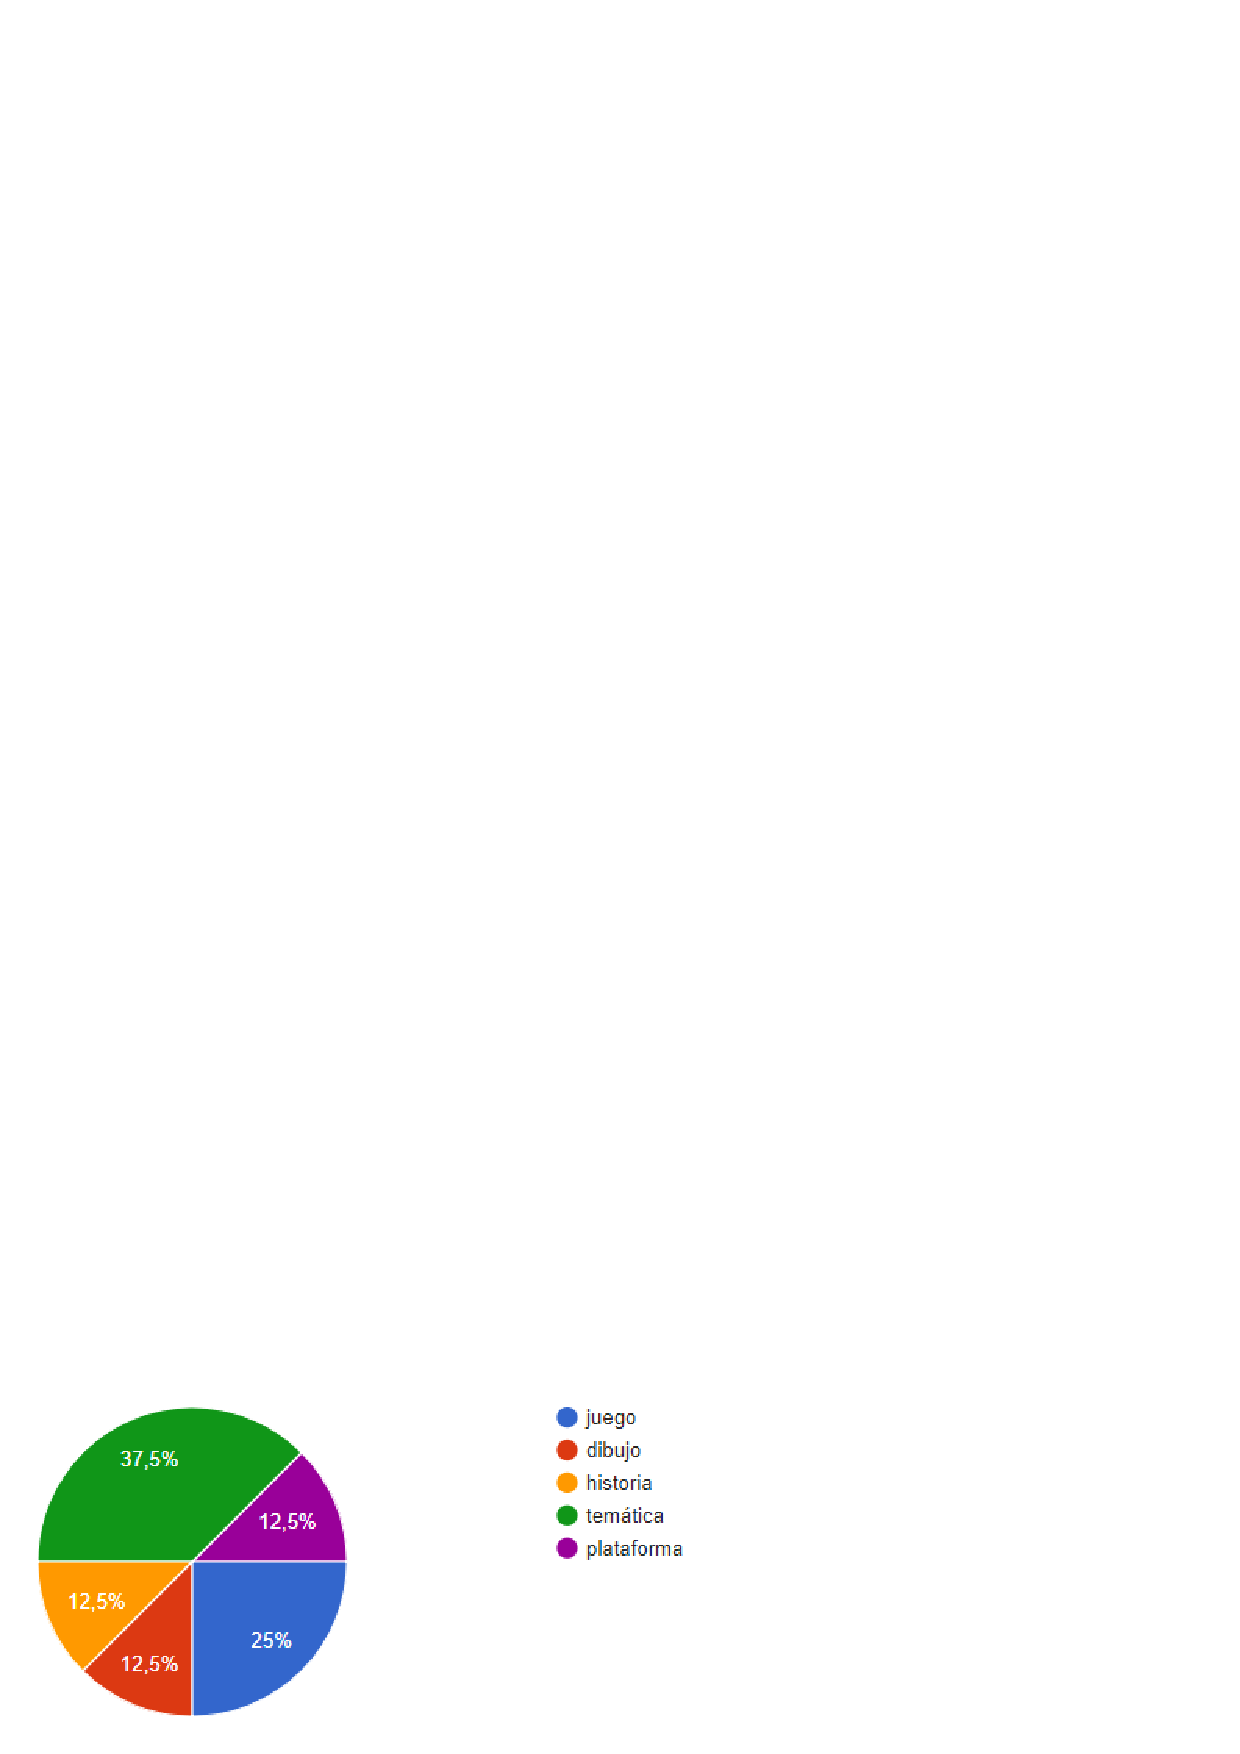
\includegraphics[width=0.5\textwidth]{04ResultadosObetnidos/pruebaR/imagenes/que/pos03}
\end{figure}


	 ¿Qué dificultad encontraste al jugar?
	Respuesta: Los encuestados en su mayoría contestaron sobre los movimientos o acciones que se podían realizar dentro del juego, que asu percepción parecían aveces impredecibles.

 ¿Que cambiarías del juego?
	Respuesta: Los usuarios en su mayoria mencionan sobre una mayor interacción en el juego sobre el personaje a otras acciones o eventos. 
	

	¿Qué senimiento tienes? 
	\begin{itemize}
		\item Alegría
		\item Enojo
		\item Tristeza
		\item Curiosidad
		\item Fatiga
		\item Otro?
	\end{itemize}

\begin{figure}
	\centering
	\caption{Gráfica de sentimiento}
	\label{fig:pos04}
	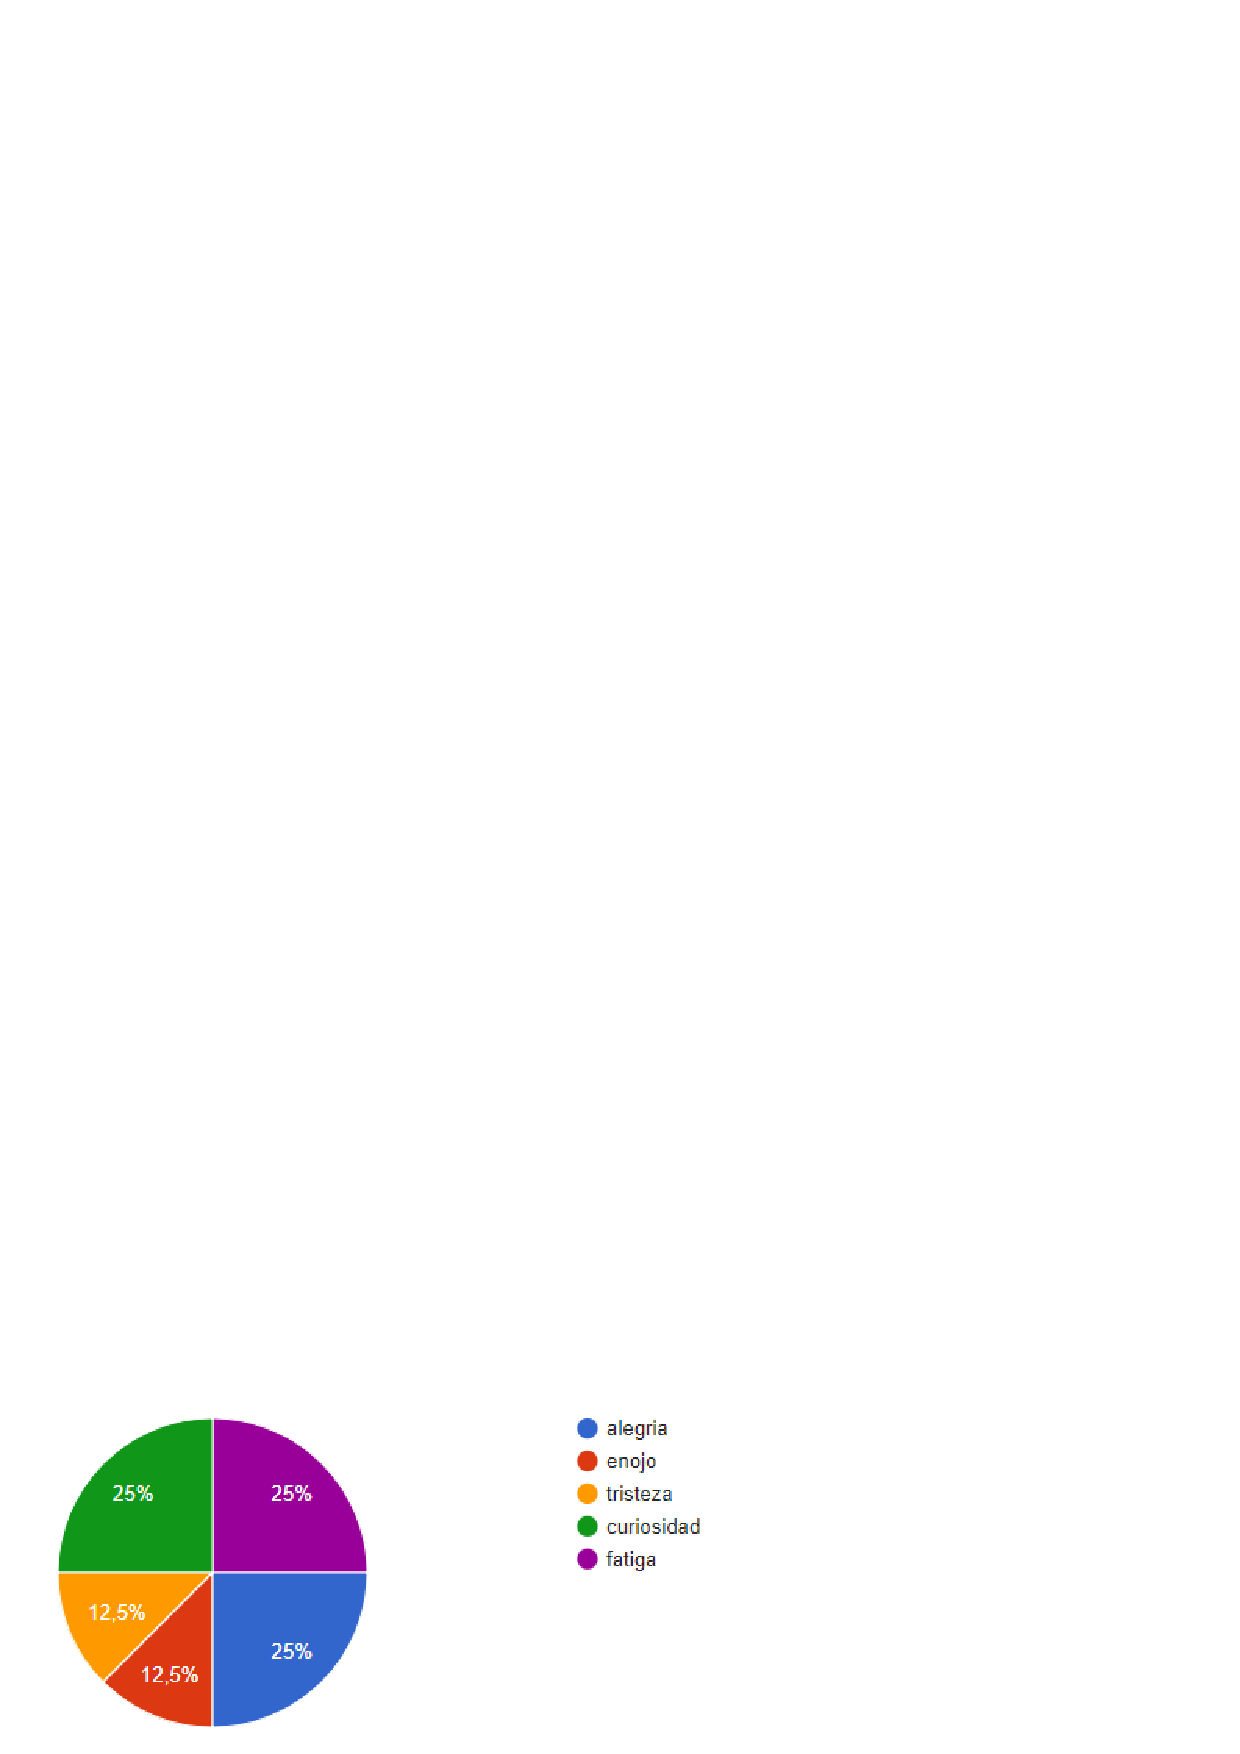
\includegraphics[width=0.5\textwidth]{04ResultadosObetnidos/pruebaR/imagenes/que/pos04}
\end{figure}



	Pirámide emocional. ¿En que escalón te encuestras ahora?
	%%poner imagen
	Respuesta: La mayoría de los jugadores seguía en el estado de seguridad o tranquilidad después del juego y seguidos de ellos algunos presentaban una emoción de autorrealización.



\section{Niveles terminados}
Para que un nivel pueda ser considerado terminado debe de tener al menos la 
funcionalidad especificada en el documento de diseño, la cual contempla lo 
siguiente: 
\begin{itemize}
        \item Actualización de la barra de vida.
        \item Actualización de la barra de \textit{tonalli}
        \item Actualización de los marcadores, en caso de que el nivel contenga objetos 
        coleccionables.
        \item Enemigos, salvo por el primer nivel.
        \item Obstáculos.
        \item Ítems, salvo por el primer nivel.
        \item Control del personaje por medio de la \textit{GUI}.
        \item Gestión de la muerte del jugador.
        \item Puntos de guardado.
\end{itemize} 

En la figura \ref{fig:NivelesPares} se muestra la funcionalidad con la que cuentan los niveles pares.
		
		\begin{figure}[h]
    			\centering
    			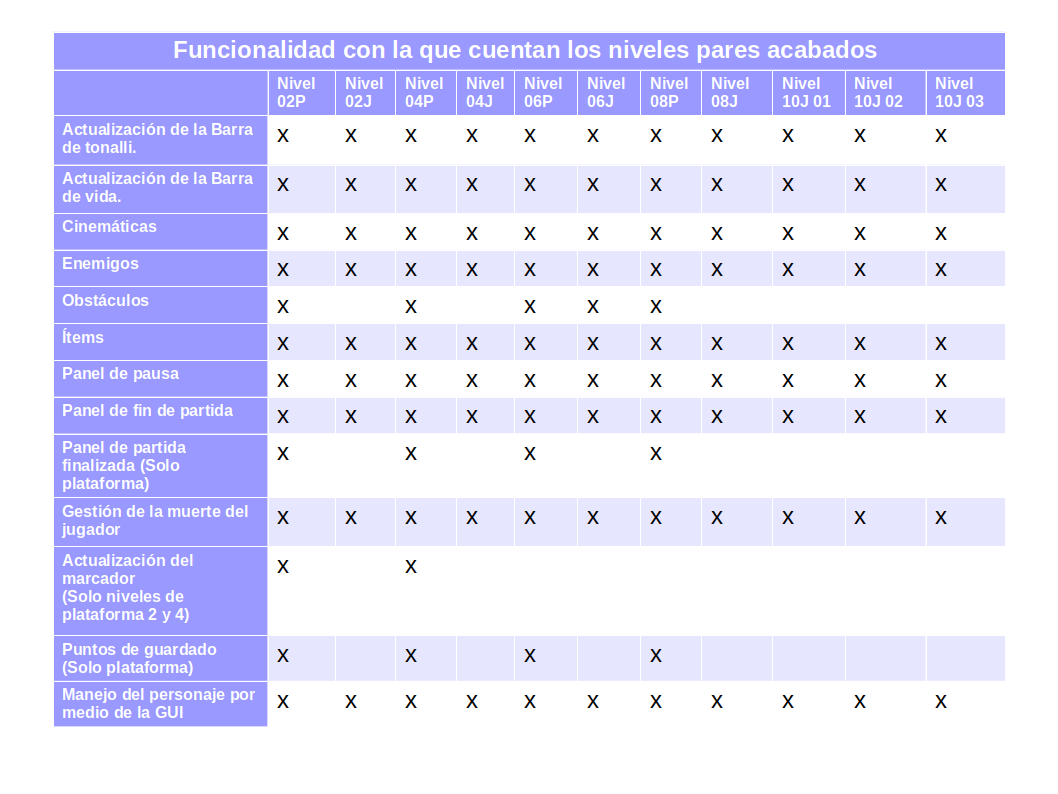
\includegraphics[width=0.9\textwidth]{04ResultadosObetnidos/imagenes/funcionalidadPares.png}
    			\caption{Funcionalidad con la que cuentan los niveles pares, la P es 
    			para los niveles de plataforma y la J para los niveles de jefes.}
    			\label{fig:NivelesPares}
		\end{figure}
